% Created by tikzDevice version 0.12.3 on 2020-02-03 16:11:50
% !TEX encoding = UTF-8 Unicode
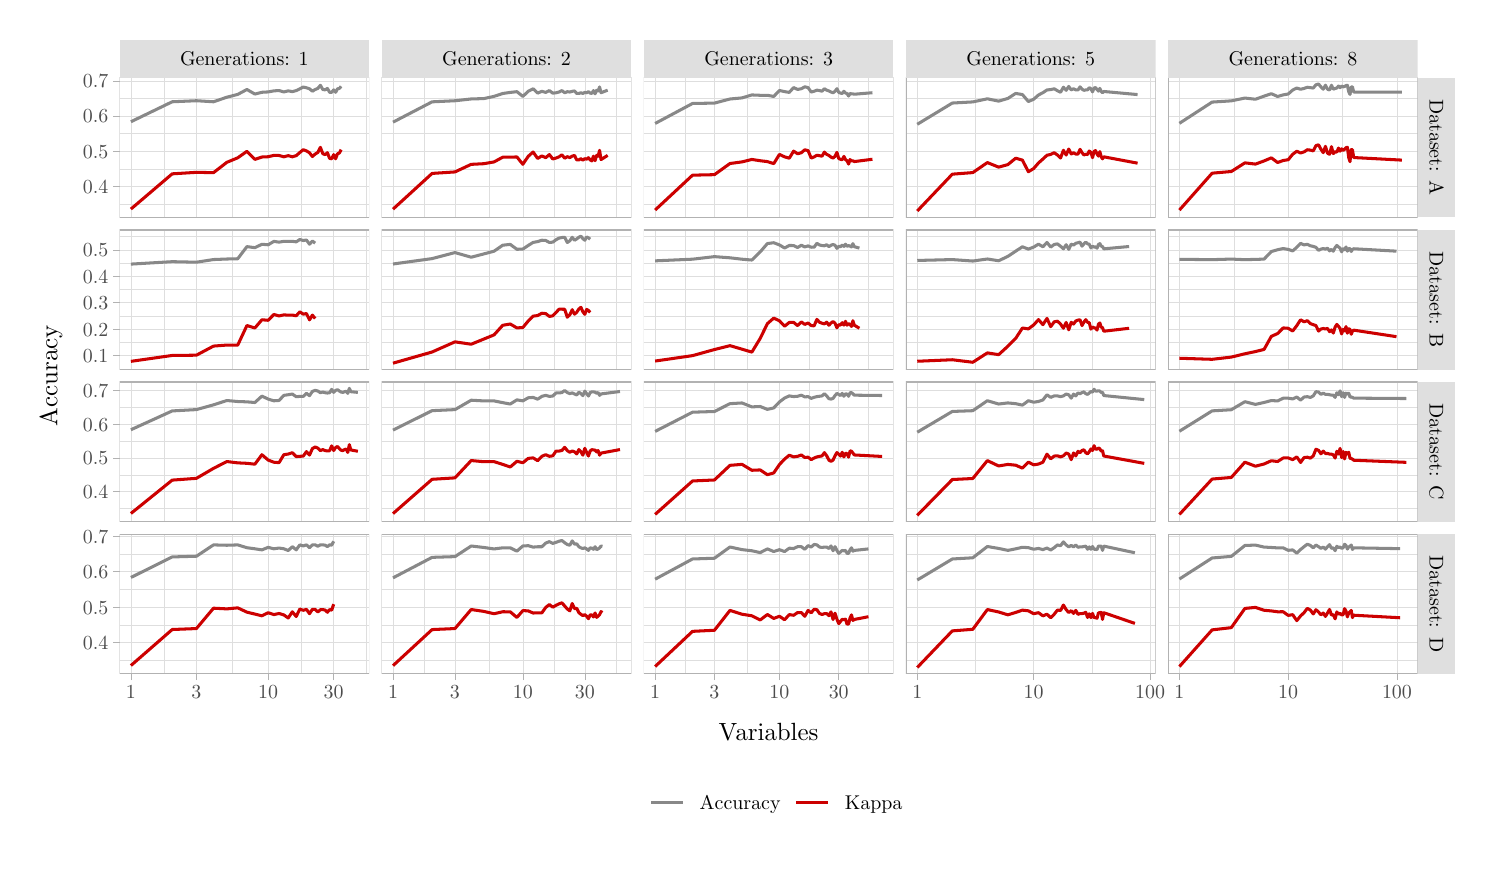
\begin{tikzpicture}[x=1pt,y=1pt]
\definecolor{fillColor}{RGB}{255,255,255}
\path[use as bounding box,fill=fillColor,fill opacity=0.00] (0,0) rectangle (520.34,296.31);
\begin{scope}
\path[clip] (  0.00,  0.00) rectangle (520.34,296.31);
\definecolor{drawColor}{RGB}{255,255,255}
\definecolor{fillColor}{RGB}{255,255,255}

\path[draw=drawColor,line width= 0.5pt,line join=round,line cap=round,fill=fillColor] ( -0.00,  0.00) rectangle (520.34,296.31);
\end{scope}
\begin{scope}
\path[clip] ( 33.20,227.76) rectangle (123.41,278.25);
\definecolor{fillColor}{RGB}{255,255,255}

\path[fill=fillColor] ( 33.20,227.76) rectangle (123.41,278.25);
\definecolor{drawColor}{gray}{0.87}

\path[draw=drawColor,line width= 0.1pt,line join=round] ( 33.20,232.64) --
	(123.41,232.64);

\path[draw=drawColor,line width= 0.1pt,line join=round] ( 33.20,245.33) --
	(123.41,245.33);

\path[draw=drawColor,line width= 0.1pt,line join=round] ( 33.20,258.03) --
	(123.41,258.03);

\path[draw=drawColor,line width= 0.1pt,line join=round] ( 33.20,270.72) --
	(123.41,270.72);

\path[draw=drawColor,line width= 0.1pt,line join=round] ( 49.13,227.76) --
	( 49.13,278.25);

\path[draw=drawColor,line width= 0.1pt,line join=round] ( 73.94,227.76) --
	( 73.94,278.25);

\path[draw=drawColor,line width= 0.1pt,line join=round] ( 98.74,227.76) --
	( 98.74,278.25);

\path[draw=drawColor,line width= 0.1pt,line join=round] (122.41,227.76) --
	(122.41,278.25);

\path[draw=drawColor,line width= 0.2pt,line join=round] ( 33.20,238.99) --
	(123.41,238.99);

\path[draw=drawColor,line width= 0.2pt,line join=round] ( 33.20,251.68) --
	(123.41,251.68);

\path[draw=drawColor,line width= 0.2pt,line join=round] ( 33.20,264.37) --
	(123.41,264.37);

\path[draw=drawColor,line width= 0.2pt,line join=round] ( 33.20,277.06) --
	(123.41,277.06);

\path[draw=drawColor,line width= 0.2pt,line join=round] ( 37.30,227.76) --
	( 37.30,278.25);

\path[draw=drawColor,line width= 0.2pt,line join=round] ( 60.97,227.76) --
	( 60.97,278.25);

\path[draw=drawColor,line width= 0.2pt,line join=round] ( 86.91,227.76) --
	( 86.91,278.25);

\path[draw=drawColor,line width= 0.2pt,line join=round] (110.58,227.76) --
	(110.58,278.25);
\definecolor{drawColor}{RGB}{136,136,136}

\path[draw=drawColor,line width= 1.1pt,line join=round] ( 37.30,262.31) --
	( 52.23,269.53) --
	( 60.97,269.91) --
	( 67.16,269.53) --
	( 71.97,271.18) --
	( 75.90,272.19) --
	( 79.22,273.97) --
	( 82.10,272.32) --
	( 84.64,272.96) --
	( 86.91,273.09) --
	( 88.96,273.47) --
	( 90.84,273.59) --
	( 92.56,273.08) --
	( 94.16,273.47) --
	( 95.64,273.20) --
	( 97.03,273.57) --
	( 98.34,274.21) --
	( 99.57,274.85) --
	(100.74,274.59) --
	(101.84,274.22) --
	(102.89,273.34) --
	(103.89,273.97) --
	(104.85,274.35) --
	(105.77,275.49) --
	(106.65,273.96) --
	(107.49,273.84) --
	(108.31,274.35) --
	(109.09,272.97) --
	(109.85,272.95) --
	(110.58,273.84) --
	(111.28,272.96) --
	(111.97,274.22) --
	(112.63,274.35) --
	(113.27,275.11);
\definecolor{drawColor}{RGB}{204,0,0}

\path[draw=drawColor,line width= 1.1pt,line join=round] ( 37.30,230.76) --
	( 52.23,243.49) --
	( 60.97,244.03) --
	( 67.16,243.92) --
	( 71.97,247.65) --
	( 75.90,249.28) --
	( 79.22,251.62) --
	( 82.10,248.72) --
	( 84.64,249.57) --
	( 86.91,249.67) --
	( 88.96,250.16) --
	( 90.84,250.12) --
	( 92.56,249.64) --
	( 94.16,250.07) --
	( 95.64,249.65) --
	( 97.03,250.06) --
	( 98.34,251.19) --
	( 99.57,252.22) --
	(100.74,251.77) --
	(101.84,251.10) --
	(102.89,249.74) --
	(103.89,250.65) --
	(104.85,251.21) --
	(105.77,253.07) --
	(106.65,250.75) --
	(107.49,250.44) --
	(108.31,251.13) --
	(109.09,249.07) --
	(109.85,248.92) --
	(110.58,250.44) --
	(111.28,248.92) --
	(111.97,250.77) --
	(112.63,250.99) --
	(113.27,252.25);
\definecolor{drawColor}{gray}{0.70}

\path[draw=drawColor,line width= 0.5pt,line join=round,line cap=round] ( 33.20,227.76) rectangle (123.41,278.25);
\end{scope}
\begin{scope}
\path[clip] ( 33.20,172.78) rectangle (123.41,223.26);
\definecolor{fillColor}{RGB}{255,255,255}

\path[fill=fillColor] ( 33.20,172.78) rectangle (123.41,223.26);
\definecolor{drawColor}{gray}{0.87}

\path[draw=drawColor,line width= 0.1pt,line join=round] ( 33.20,173.04) --
	(123.41,173.04);

\path[draw=drawColor,line width= 0.1pt,line join=round] ( 33.20,182.59) --
	(123.41,182.59);

\path[draw=drawColor,line width= 0.1pt,line join=round] ( 33.20,192.14) --
	(123.41,192.14);

\path[draw=drawColor,line width= 0.1pt,line join=round] ( 33.20,201.70) --
	(123.41,201.70);

\path[draw=drawColor,line width= 0.1pt,line join=round] ( 33.20,211.25) --
	(123.41,211.25);

\path[draw=drawColor,line width= 0.1pt,line join=round] ( 33.20,220.80) --
	(123.41,220.80);

\path[draw=drawColor,line width= 0.1pt,line join=round] ( 49.13,172.78) --
	( 49.13,223.26);

\path[draw=drawColor,line width= 0.1pt,line join=round] ( 73.94,172.78) --
	( 73.94,223.26);

\path[draw=drawColor,line width= 0.1pt,line join=round] ( 98.74,172.78) --
	( 98.74,223.26);

\path[draw=drawColor,line width= 0.1pt,line join=round] (122.41,172.78) --
	(122.41,223.26);

\path[draw=drawColor,line width= 0.2pt,line join=round] ( 33.20,177.81) --
	(123.41,177.81);

\path[draw=drawColor,line width= 0.2pt,line join=round] ( 33.20,187.37) --
	(123.41,187.37);

\path[draw=drawColor,line width= 0.2pt,line join=round] ( 33.20,196.92) --
	(123.41,196.92);

\path[draw=drawColor,line width= 0.2pt,line join=round] ( 33.20,206.47) --
	(123.41,206.47);

\path[draw=drawColor,line width= 0.2pt,line join=round] ( 33.20,216.03) --
	(123.41,216.03);

\path[draw=drawColor,line width= 0.2pt,line join=round] ( 37.30,172.78) --
	( 37.30,223.26);

\path[draw=drawColor,line width= 0.2pt,line join=round] ( 60.97,172.78) --
	( 60.97,223.26);

\path[draw=drawColor,line width= 0.2pt,line join=round] ( 86.91,172.78) --
	( 86.91,223.26);

\path[draw=drawColor,line width= 0.2pt,line join=round] (110.58,172.78) --
	(110.58,223.26);
\definecolor{drawColor}{RGB}{136,136,136}

\path[draw=drawColor,line width= 1.1pt,line join=round] ( 37.30,210.87) --
	( 52.23,211.75) --
	( 60.97,211.56) --
	( 67.16,212.52) --
	( 71.97,212.71) --
	( 75.90,212.81) --
	( 79.22,217.19) --
	( 82.10,216.81) --
	( 84.64,218.04) --
	( 86.91,217.85) --
	( 88.96,219.09) --
	( 90.84,218.81) --
	( 92.56,219.10) --
	( 94.16,219.10) --
	( 95.64,219.10) --
	( 97.03,218.91) --
	( 98.34,219.77) --
	( 99.57,219.39) --
	(100.74,219.58) --
	(101.84,218.06) --
	(102.89,219.20) --
	(103.89,218.44);
\definecolor{drawColor}{RGB}{204,0,0}

\path[draw=drawColor,line width= 1.1pt,line join=round] ( 37.30,175.73) --
	( 52.23,177.86) --
	( 60.97,177.96) --
	( 67.16,181.25) --
	( 71.97,181.62) --
	( 75.90,181.59) --
	( 79.22,188.68) --
	( 82.10,187.79) --
	( 84.64,190.76) --
	( 86.91,190.57) --
	( 88.96,192.68) --
	( 90.84,192.14) --
	( 92.56,192.52) --
	( 94.16,192.43) --
	( 95.64,192.45) --
	( 97.03,192.20) --
	( 98.34,193.64) --
	( 99.57,192.79) --
	(100.74,193.00) --
	(101.84,190.72) --
	(102.89,192.45) --
	(103.89,191.20);
\definecolor{drawColor}{gray}{0.70}

\path[draw=drawColor,line width= 0.5pt,line join=round,line cap=round] ( 33.20,172.78) rectangle (123.41,223.26);
\end{scope}
\begin{scope}
\path[clip] ( 33.20,117.79) rectangle (123.41,168.28);
\definecolor{fillColor}{RGB}{255,255,255}

\path[fill=fillColor] ( 33.20,117.79) rectangle (123.41,168.28);
\definecolor{drawColor}{gray}{0.87}

\path[draw=drawColor,line width= 0.1pt,line join=round] ( 33.20,122.57) --
	(123.41,122.57);

\path[draw=drawColor,line width= 0.1pt,line join=round] ( 33.20,134.74) --
	(123.41,134.74);

\path[draw=drawColor,line width= 0.1pt,line join=round] ( 33.20,146.91) --
	(123.41,146.91);

\path[draw=drawColor,line width= 0.1pt,line join=round] ( 33.20,159.08) --
	(123.41,159.08);

\path[draw=drawColor,line width= 0.1pt,line join=round] ( 49.13,117.79) --
	( 49.13,168.28);

\path[draw=drawColor,line width= 0.1pt,line join=round] ( 73.94,117.79) --
	( 73.94,168.28);

\path[draw=drawColor,line width= 0.1pt,line join=round] ( 98.74,117.79) --
	( 98.74,168.28);

\path[draw=drawColor,line width= 0.1pt,line join=round] (122.41,117.79) --
	(122.41,168.28);

\path[draw=drawColor,line width= 0.2pt,line join=round] ( 33.20,128.65) --
	(123.41,128.65);

\path[draw=drawColor,line width= 0.2pt,line join=round] ( 33.20,140.82) --
	(123.41,140.82);

\path[draw=drawColor,line width= 0.2pt,line join=round] ( 33.20,152.99) --
	(123.41,152.99);

\path[draw=drawColor,line width= 0.2pt,line join=round] ( 33.20,165.16) --
	(123.41,165.16);

\path[draw=drawColor,line width= 0.2pt,line join=round] ( 37.30,117.79) --
	( 37.30,168.28);

\path[draw=drawColor,line width= 0.2pt,line join=round] ( 60.97,117.79) --
	( 60.97,168.28);

\path[draw=drawColor,line width= 0.2pt,line join=round] ( 86.91,117.79) --
	( 86.91,168.28);

\path[draw=drawColor,line width= 0.2pt,line join=round] (110.58,117.79) --
	(110.58,168.28);
\definecolor{drawColor}{RGB}{136,136,136}

\path[draw=drawColor,line width= 1.1pt,line join=round] ( 37.30,151.02) --
	( 52.23,157.82) --
	( 60.97,158.30) --
	( 67.16,160.02) --
	( 71.97,161.58) --
	( 75.90,161.22) --
	( 79.22,161.10) --
	( 82.10,160.86) --
	( 84.64,163.18) --
	( 86.91,162.09) --
	( 88.96,161.48) --
	( 90.84,161.61) --
	( 92.56,163.44) --
	( 94.16,163.67) --
	( 95.64,163.92) --
	( 97.03,162.95) --
	( 98.34,163.07) --
	( 99.57,163.07) --
	(100.74,164.17) --
	(101.84,163.32) --
	(102.89,164.88) --
	(103.89,165.25) --
	(104.85,165.01) --
	(105.77,164.40) --
	(106.65,164.64) --
	(107.49,164.40) --
	(108.31,164.28) --
	(109.09,164.40) --
	(109.85,165.61) --
	(110.58,164.52) --
	(111.28,165.25) --
	(111.97,165.49) --
	(112.63,165.01) --
	(113.27,164.64) --
	(113.90,164.52) --
	(114.51,164.77) --
	(115.10,164.90) --
	(115.67,164.16) --
	(116.23,165.98) --
	(116.78,164.77) --
	(119.31,164.52);
\definecolor{drawColor}{RGB}{204,0,0}

\path[draw=drawColor,line width= 1.1pt,line join=round] ( 37.30,120.76) --
	( 52.23,132.82) --
	( 60.97,133.46) --
	( 67.16,137.07) --
	( 71.97,139.53) --
	( 75.90,139.05) --
	( 79.22,138.89) --
	( 82.10,138.57) --
	( 84.64,142.00) --
	( 86.91,140.06) --
	( 88.96,139.28) --
	( 90.84,139.13) --
	( 92.56,142.00) --
	( 94.16,142.24) --
	( 95.64,142.73) --
	( 97.03,141.32) --
	( 98.34,141.42) --
	( 99.57,141.49) --
	(100.74,143.12) --
	(101.84,141.87) --
	(102.89,144.22) --
	(103.89,144.80) --
	(104.85,144.36) --
	(105.77,143.47) --
	(106.65,143.86) --
	(107.49,143.48) --
	(108.31,143.36) --
	(109.09,143.44) --
	(109.85,145.20) --
	(110.58,143.51) --
	(111.28,144.61) --
	(111.97,144.96) --
	(112.63,144.18) --
	(113.27,143.60) --
	(113.90,143.47) --
	(114.51,143.87) --
	(115.10,144.01) --
	(115.67,142.81) --
	(116.23,145.64) --
	(116.78,143.71) --
	(119.31,143.24);
\definecolor{drawColor}{gray}{0.70}

\path[draw=drawColor,line width= 0.5pt,line join=round,line cap=round] ( 33.20,117.79) rectangle (123.41,168.28);
\end{scope}
\begin{scope}
\path[clip] ( 33.20, 62.81) rectangle (123.41,113.29);
\definecolor{fillColor}{RGB}{255,255,255}

\path[fill=fillColor] ( 33.20, 62.81) rectangle (123.41,113.29);
\definecolor{drawColor}{gray}{0.87}

\path[draw=drawColor,line width= 0.1pt,line join=round] ( 33.20, 67.71) --
	(123.41, 67.71);

\path[draw=drawColor,line width= 0.1pt,line join=round] ( 33.20, 80.52) --
	(123.41, 80.52);

\path[draw=drawColor,line width= 0.1pt,line join=round] ( 33.20, 93.32) --
	(123.41, 93.32);

\path[draw=drawColor,line width= 0.1pt,line join=round] ( 33.20,106.13) --
	(123.41,106.13);

\path[draw=drawColor,line width= 0.1pt,line join=round] ( 49.13, 62.81) --
	( 49.13,113.29);

\path[draw=drawColor,line width= 0.1pt,line join=round] ( 73.94, 62.81) --
	( 73.94,113.29);

\path[draw=drawColor,line width= 0.1pt,line join=round] ( 98.74, 62.81) --
	( 98.74,113.29);

\path[draw=drawColor,line width= 0.1pt,line join=round] (122.41, 62.81) --
	(122.41,113.29);

\path[draw=drawColor,line width= 0.2pt,line join=round] ( 33.20, 74.12) --
	(123.41, 74.12);

\path[draw=drawColor,line width= 0.2pt,line join=round] ( 33.20, 86.92) --
	(123.41, 86.92);

\path[draw=drawColor,line width= 0.2pt,line join=round] ( 33.20, 99.73) --
	(123.41, 99.73);

\path[draw=drawColor,line width= 0.2pt,line join=round] ( 33.20,112.53) --
	(123.41,112.53);

\path[draw=drawColor,line width= 0.2pt,line join=round] ( 37.30, 62.81) --
	( 37.30,113.29);

\path[draw=drawColor,line width= 0.2pt,line join=round] ( 60.97, 62.81) --
	( 60.97,113.29);

\path[draw=drawColor,line width= 0.2pt,line join=round] ( 86.91, 62.81) --
	( 86.91,113.29);

\path[draw=drawColor,line width= 0.2pt,line join=round] (110.58, 62.81) --
	(110.58,113.29);
\definecolor{drawColor}{RGB}{136,136,136}

\path[draw=drawColor,line width= 1.1pt,line join=round] ( 37.30, 97.64) --
	( 52.23,105.06) --
	( 60.97,105.31) --
	( 67.16,109.41) --
	( 71.97,109.28) --
	( 75.90,109.41) --
	( 79.22,108.39) --
	( 82.10,108.00) --
	( 84.64,107.61) --
	( 86.91,108.52) --
	( 88.96,108.00) --
	( 90.84,108.27) --
	( 92.56,108.01) --
	( 94.16,107.37) --
	( 95.64,108.78) --
	( 97.03,107.63) --
	( 98.34,109.42) --
	( 99.57,109.04) --
	(100.74,109.42) --
	(101.84,108.40) --
	(102.89,109.42) --
	(103.89,109.43) --
	(104.85,108.92) --
	(105.77,109.43) --
	(106.65,109.43) --
	(107.49,109.30) --
	(108.31,108.80) --
	(109.09,109.44) --
	(109.85,109.30) --
	(110.58,110.71);
\definecolor{drawColor}{RGB}{204,0,0}

\path[draw=drawColor,line width= 1.1pt,line join=round] ( 37.30, 65.81) --
	( 52.23, 78.83) --
	( 60.97, 79.18) --
	( 67.16, 86.54) --
	( 71.97, 86.29) --
	( 75.90, 86.66) --
	( 79.22, 85.11) --
	( 82.10, 84.41) --
	( 84.64, 83.79) --
	( 86.91, 84.90) --
	( 88.96, 84.23) --
	( 90.84, 84.63) --
	( 92.56, 84.10) --
	( 94.16, 83.00) --
	( 95.64, 85.24) --
	( 97.03, 83.53) --
	( 98.34, 86.24) --
	( 99.57, 85.77) --
	(100.74, 86.13) --
	(101.84, 84.55) --
	(102.89, 86.13) --
	(103.89, 86.10) --
	(104.85, 85.19) --
	(105.77, 85.98) --
	(106.65, 86.03) --
	(107.49, 85.86) --
	(108.31, 85.07) --
	(109.09, 86.03) --
	(109.85, 85.82) --
	(110.58, 87.98);
\definecolor{drawColor}{gray}{0.70}

\path[draw=drawColor,line width= 0.5pt,line join=round,line cap=round] ( 33.20, 62.81) rectangle (123.41,113.29);
\end{scope}
\begin{scope}
\path[clip] (127.91,227.76) rectangle (218.13,278.25);
\definecolor{fillColor}{RGB}{255,255,255}

\path[fill=fillColor] (127.91,227.76) rectangle (218.13,278.25);
\definecolor{drawColor}{gray}{0.87}

\path[draw=drawColor,line width= 0.1pt,line join=round] (127.91,232.64) --
	(218.13,232.64);

\path[draw=drawColor,line width= 0.1pt,line join=round] (127.91,245.33) --
	(218.13,245.33);

\path[draw=drawColor,line width= 0.1pt,line join=round] (127.91,258.03) --
	(218.13,258.03);

\path[draw=drawColor,line width= 0.1pt,line join=round] (127.91,270.72) --
	(218.13,270.72);

\path[draw=drawColor,line width= 0.1pt,line join=round] (143.21,227.76) --
	(143.21,278.25);

\path[draw=drawColor,line width= 0.1pt,line join=round] (166.66,227.76) --
	(166.66,278.25);

\path[draw=drawColor,line width= 0.1pt,line join=round] (190.12,227.76) --
	(190.12,278.25);

\path[draw=drawColor,line width= 0.1pt,line join=round] (212.51,227.76) --
	(212.51,278.25);

\path[draw=drawColor,line width= 0.2pt,line join=round] (127.91,238.99) --
	(218.13,238.99);

\path[draw=drawColor,line width= 0.2pt,line join=round] (127.91,251.68) --
	(218.13,251.68);

\path[draw=drawColor,line width= 0.2pt,line join=round] (127.91,264.37) --
	(218.13,264.37);

\path[draw=drawColor,line width= 0.2pt,line join=round] (127.91,277.06) --
	(218.13,277.06);

\path[draw=drawColor,line width= 0.2pt,line join=round] (132.01,227.76) --
	(132.01,278.25);

\path[draw=drawColor,line width= 0.2pt,line join=round] (154.40,227.76) --
	(154.40,278.25);

\path[draw=drawColor,line width= 0.2pt,line join=round] (178.93,227.76) --
	(178.93,278.25);

\path[draw=drawColor,line width= 0.2pt,line join=round] (201.31,227.76) --
	(201.31,278.25);
\definecolor{drawColor}{RGB}{136,136,136}

\path[draw=drawColor,line width= 1.1pt,line join=round] (132.01,262.16) --
	(146.14,269.51) --
	(154.40,269.90) --
	(160.26,270.55) --
	(164.81,270.68) --
	(168.52,271.48) --
	(171.66,272.52) --
	(174.38,272.91) --
	(176.78,273.18) --
	(178.93,271.47) --
	(180.87,273.31) --
	(182.64,274.23) --
	(184.28,272.66) --
	(185.79,273.31) --
	(187.19,272.92) --
	(188.51,273.57) --
	(189.74,272.65) --
	(190.91,272.78) --
	(192.01,273.05) --
	(193.05,273.58) --
	(194.05,272.79) --
	(194.99,273.18) --
	(195.90,273.05) --
	(196.77,273.31) --
	(197.60,273.44) --
	(198.40,272.53) --
	(199.17,272.53) --
	(199.91,272.79) --
	(200.62,272.53) --
	(201.31,272.92) --
	(201.98,272.78) --
	(202.63,273.18) --
	(203.26,272.66) --
	(203.86,272.53) --
	(204.45,273.58) --
	(205.03,272.41) --
	(205.59,273.71) --
	(206.13,273.45) --
	(206.66,274.89) --
	(207.18,272.80) --
	(209.58,273.72);
\definecolor{drawColor}{RGB}{204,0,0}

\path[draw=drawColor,line width= 1.1pt,line join=round] (132.01,230.72) --
	(146.14,243.64) --
	(154.40,244.18) --
	(160.26,246.92) --
	(164.81,247.15) --
	(168.52,247.80) --
	(171.66,249.50) --
	(174.38,249.50) --
	(176.78,249.60) --
	(178.93,246.94) --
	(180.87,249.82) --
	(182.64,251.38) --
	(184.28,249.04) --
	(185.79,249.97) --
	(187.19,249.32) --
	(188.51,250.45) --
	(189.74,248.86) --
	(190.91,249.20) --
	(192.01,249.63) --
	(193.05,250.38) --
	(194.05,249.13) --
	(194.99,249.71) --
	(195.90,249.35) --
	(196.77,249.89) --
	(197.60,250.14) --
	(198.40,248.53) --
	(199.17,248.51) --
	(199.91,248.95) --
	(200.62,248.43) --
	(201.31,248.98) --
	(201.98,248.76) --
	(202.63,249.31) --
	(203.26,248.52) --
	(203.86,248.16) --
	(204.45,249.89) --
	(205.03,248.24) --
	(205.59,250.17) --
	(206.13,249.82) --
	(206.66,252.00) --
	(207.18,248.64) --
	(209.58,250.16);
\definecolor{drawColor}{gray}{0.70}

\path[draw=drawColor,line width= 0.5pt,line join=round,line cap=round] (127.91,227.76) rectangle (218.13,278.25);
\end{scope}
\begin{scope}
\path[clip] (127.91,172.78) rectangle (218.13,223.26);
\definecolor{fillColor}{RGB}{255,255,255}

\path[fill=fillColor] (127.91,172.78) rectangle (218.13,223.26);
\definecolor{drawColor}{gray}{0.87}

\path[draw=drawColor,line width= 0.1pt,line join=round] (127.91,173.04) --
	(218.13,173.04);

\path[draw=drawColor,line width= 0.1pt,line join=round] (127.91,182.59) --
	(218.13,182.59);

\path[draw=drawColor,line width= 0.1pt,line join=round] (127.91,192.14) --
	(218.13,192.14);

\path[draw=drawColor,line width= 0.1pt,line join=round] (127.91,201.70) --
	(218.13,201.70);

\path[draw=drawColor,line width= 0.1pt,line join=round] (127.91,211.25) --
	(218.13,211.25);

\path[draw=drawColor,line width= 0.1pt,line join=round] (127.91,220.80) --
	(218.13,220.80);

\path[draw=drawColor,line width= 0.1pt,line join=round] (143.21,172.78) --
	(143.21,223.26);

\path[draw=drawColor,line width= 0.1pt,line join=round] (166.66,172.78) --
	(166.66,223.26);

\path[draw=drawColor,line width= 0.1pt,line join=round] (190.12,172.78) --
	(190.12,223.26);

\path[draw=drawColor,line width= 0.1pt,line join=round] (212.51,172.78) --
	(212.51,223.26);

\path[draw=drawColor,line width= 0.2pt,line join=round] (127.91,177.81) --
	(218.13,177.81);

\path[draw=drawColor,line width= 0.2pt,line join=round] (127.91,187.37) --
	(218.13,187.37);

\path[draw=drawColor,line width= 0.2pt,line join=round] (127.91,196.92) --
	(218.13,196.92);

\path[draw=drawColor,line width= 0.2pt,line join=round] (127.91,206.47) --
	(218.13,206.47);

\path[draw=drawColor,line width= 0.2pt,line join=round] (127.91,216.03) --
	(218.13,216.03);

\path[draw=drawColor,line width= 0.2pt,line join=round] (132.01,172.78) --
	(132.01,223.26);

\path[draw=drawColor,line width= 0.2pt,line join=round] (154.40,172.78) --
	(154.40,223.26);

\path[draw=drawColor,line width= 0.2pt,line join=round] (178.93,172.78) --
	(178.93,223.26);

\path[draw=drawColor,line width= 0.2pt,line join=round] (201.31,172.78) --
	(201.31,223.26);
\definecolor{drawColor}{RGB}{136,136,136}

\path[draw=drawColor,line width= 1.1pt,line join=round] (132.01,210.91) --
	(146.14,212.86) --
	(154.40,215.04) --
	(160.26,213.36) --
	(164.81,214.55) --
	(168.52,215.53) --
	(171.66,217.70) --
	(174.38,218.00) --
	(176.78,216.22) --
	(178.93,216.32) --
	(180.87,217.61) --
	(182.64,218.71) --
	(184.28,219.00) --
	(185.79,219.50) --
	(187.19,219.40) --
	(188.51,218.71) --
	(189.74,218.80) --
	(190.91,219.68) --
	(192.01,220.27) --
	(193.05,220.48) --
	(194.05,220.57) --
	(194.99,218.69) --
	(195.90,219.29) --
	(196.77,220.57) --
	(197.60,219.49) --
	(198.40,219.98) --
	(199.17,220.57) --
	(199.91,220.97) --
	(200.62,220.08) --
	(201.31,219.49) --
	(201.98,220.67) --
	(202.63,220.38) --
	(203.26,219.88);
\definecolor{drawColor}{RGB}{204,0,0}

\path[draw=drawColor,line width= 1.1pt,line join=round] (132.01,175.07) --
	(146.14,179.11) --
	(154.40,182.78) --
	(160.26,181.92) --
	(164.81,183.78) --
	(168.52,185.30) --
	(171.66,188.76) --
	(174.38,189.23) --
	(176.78,187.82) --
	(178.93,187.96) --
	(180.87,190.30) --
	(182.64,192.07) --
	(184.28,192.29) --
	(185.79,193.12) --
	(187.19,192.99) --
	(188.51,191.97) --
	(189.74,192.18) --
	(190.91,193.39) --
	(192.01,194.58) --
	(193.05,194.57) --
	(194.05,194.55) --
	(194.99,191.69) --
	(195.90,192.55) --
	(196.77,194.41) --
	(197.60,192.78) --
	(198.40,193.46) --
	(199.17,194.66) --
	(199.91,195.26) --
	(200.62,193.65) --
	(201.31,192.72) --
	(201.98,194.51) --
	(202.63,194.12) --
	(203.26,193.41);
\definecolor{drawColor}{gray}{0.70}

\path[draw=drawColor,line width= 0.5pt,line join=round,line cap=round] (127.91,172.78) rectangle (218.13,223.26);
\end{scope}
\begin{scope}
\path[clip] (127.91,117.79) rectangle (218.13,168.28);
\definecolor{fillColor}{RGB}{255,255,255}

\path[fill=fillColor] (127.91,117.79) rectangle (218.13,168.28);
\definecolor{drawColor}{gray}{0.87}

\path[draw=drawColor,line width= 0.1pt,line join=round] (127.91,122.57) --
	(218.13,122.57);

\path[draw=drawColor,line width= 0.1pt,line join=round] (127.91,134.74) --
	(218.13,134.74);

\path[draw=drawColor,line width= 0.1pt,line join=round] (127.91,146.91) --
	(218.13,146.91);

\path[draw=drawColor,line width= 0.1pt,line join=round] (127.91,159.08) --
	(218.13,159.08);

\path[draw=drawColor,line width= 0.1pt,line join=round] (143.21,117.79) --
	(143.21,168.28);

\path[draw=drawColor,line width= 0.1pt,line join=round] (166.66,117.79) --
	(166.66,168.28);

\path[draw=drawColor,line width= 0.1pt,line join=round] (190.12,117.79) --
	(190.12,168.28);

\path[draw=drawColor,line width= 0.1pt,line join=round] (212.51,117.79) --
	(212.51,168.28);

\path[draw=drawColor,line width= 0.2pt,line join=round] (127.91,128.65) --
	(218.13,128.65);

\path[draw=drawColor,line width= 0.2pt,line join=round] (127.91,140.82) --
	(218.13,140.82);

\path[draw=drawColor,line width= 0.2pt,line join=round] (127.91,152.99) --
	(218.13,152.99);

\path[draw=drawColor,line width= 0.2pt,line join=round] (127.91,165.16) --
	(218.13,165.16);

\path[draw=drawColor,line width= 0.2pt,line join=round] (132.01,117.79) --
	(132.01,168.28);

\path[draw=drawColor,line width= 0.2pt,line join=round] (154.40,117.79) --
	(154.40,168.28);

\path[draw=drawColor,line width= 0.2pt,line join=round] (178.93,117.79) --
	(178.93,168.28);

\path[draw=drawColor,line width= 0.2pt,line join=round] (201.31,117.79) --
	(201.31,168.28);
\definecolor{drawColor}{RGB}{136,136,136}

\path[draw=drawColor,line width= 1.1pt,line join=round] (132.01,150.88) --
	(146.14,157.92) --
	(154.40,158.29) --
	(160.26,161.69) --
	(164.81,161.44) --
	(168.52,161.44) --
	(171.66,160.81) --
	(174.38,160.31) --
	(176.78,161.82) --
	(178.93,161.45) --
	(180.87,162.57) --
	(182.64,162.70) --
	(184.28,162.07) --
	(185.79,163.08) --
	(187.19,163.45) --
	(188.51,163.07) --
	(189.74,163.19) --
	(190.91,164.32) --
	(192.01,164.32) --
	(193.05,164.45) --
	(194.05,165.21) --
	(194.99,164.45) --
	(195.90,164.08) --
	(196.77,164.33) --
	(197.60,163.95) --
	(198.40,163.58) --
	(199.17,164.59) --
	(199.91,164.08) --
	(200.62,163.33) --
	(201.31,164.96) --
	(201.98,164.08) --
	(202.63,163.20) --
	(203.26,164.46) --
	(203.86,164.71) --
	(204.45,164.71) --
	(205.03,164.59) --
	(205.59,164.21) --
	(206.13,164.47) --
	(206.66,163.45) --
	(207.18,163.96) --
	(214.03,164.84);
\definecolor{drawColor}{RGB}{204,0,0}

\path[draw=drawColor,line width= 1.1pt,line join=round] (132.01,120.72) --
	(146.14,133.11) --
	(154.40,133.63) --
	(160.26,139.89) --
	(164.81,139.47) --
	(168.52,139.50) --
	(171.66,138.50) --
	(174.38,137.56) --
	(176.78,139.62) --
	(178.93,139.10) --
	(180.87,140.66) --
	(182.64,140.86) --
	(184.28,139.83) --
	(185.79,141.41) --
	(187.19,142.02) --
	(188.51,141.41) --
	(189.74,141.59) --
	(190.91,143.31) --
	(192.01,143.31) --
	(193.05,143.52) --
	(194.05,144.67) --
	(194.99,143.47) --
	(195.90,142.88) --
	(196.77,143.35) --
	(197.60,143.04) --
	(198.40,142.28) --
	(199.17,143.85) --
	(199.91,143.07) --
	(200.62,141.84) --
	(201.31,144.31) --
	(201.98,142.84) --
	(202.63,141.52) --
	(203.26,143.36) --
	(203.86,143.82) --
	(204.45,143.74) --
	(205.03,143.65) --
	(205.59,143.00) --
	(206.13,143.51) --
	(206.66,141.81) --
	(207.18,142.58) --
	(214.03,143.86);
\definecolor{drawColor}{gray}{0.70}

\path[draw=drawColor,line width= 0.5pt,line join=round,line cap=round] (127.91,117.79) rectangle (218.13,168.28);
\end{scope}
\begin{scope}
\path[clip] (127.91, 62.81) rectangle (218.13,113.29);
\definecolor{fillColor}{RGB}{255,255,255}

\path[fill=fillColor] (127.91, 62.81) rectangle (218.13,113.29);
\definecolor{drawColor}{gray}{0.87}

\path[draw=drawColor,line width= 0.1pt,line join=round] (127.91, 67.71) --
	(218.13, 67.71);

\path[draw=drawColor,line width= 0.1pt,line join=round] (127.91, 80.52) --
	(218.13, 80.52);

\path[draw=drawColor,line width= 0.1pt,line join=round] (127.91, 93.32) --
	(218.13, 93.32);

\path[draw=drawColor,line width= 0.1pt,line join=round] (127.91,106.13) --
	(218.13,106.13);

\path[draw=drawColor,line width= 0.1pt,line join=round] (143.21, 62.81) --
	(143.21,113.29);

\path[draw=drawColor,line width= 0.1pt,line join=round] (166.66, 62.81) --
	(166.66,113.29);

\path[draw=drawColor,line width= 0.1pt,line join=round] (190.12, 62.81) --
	(190.12,113.29);

\path[draw=drawColor,line width= 0.1pt,line join=round] (212.51, 62.81) --
	(212.51,113.29);

\path[draw=drawColor,line width= 0.2pt,line join=round] (127.91, 74.12) --
	(218.13, 74.12);

\path[draw=drawColor,line width= 0.2pt,line join=round] (127.91, 86.92) --
	(218.13, 86.92);

\path[draw=drawColor,line width= 0.2pt,line join=round] (127.91, 99.73) --
	(218.13, 99.73);

\path[draw=drawColor,line width= 0.2pt,line join=round] (127.91,112.53) --
	(218.13,112.53);

\path[draw=drawColor,line width= 0.2pt,line join=round] (132.01, 62.81) --
	(132.01,113.29);

\path[draw=drawColor,line width= 0.2pt,line join=round] (154.40, 62.81) --
	(154.40,113.29);

\path[draw=drawColor,line width= 0.2pt,line join=round] (178.93, 62.81) --
	(178.93,113.29);

\path[draw=drawColor,line width= 0.2pt,line join=round] (201.31, 62.81) --
	(201.31,113.29);
\definecolor{drawColor}{RGB}{136,136,136}

\path[draw=drawColor,line width= 1.1pt,line join=round] (132.01, 97.50) --
	(146.14,104.91) --
	(154.40,105.17) --
	(160.26,109.01) --
	(164.81,108.48) --
	(168.52,107.95) --
	(171.66,108.35) --
	(174.38,108.35) --
	(176.78,107.16) --
	(178.93,109.01) --
	(180.87,109.13) --
	(182.64,108.61) --
	(184.28,108.74) --
	(185.79,108.74) --
	(187.19,110.07) --
	(188.51,110.59) --
	(189.74,109.95) --
	(190.91,110.33) --
	(192.01,110.73) --
	(193.05,111.00) --
	(194.05,110.20) --
	(194.99,109.55) --
	(195.90,109.28) --
	(196.77,110.86) --
	(197.60,109.67) --
	(198.40,109.80) --
	(199.17,108.75) --
	(199.91,108.35) --
	(200.62,108.09) --
	(201.31,108.35) --
	(201.98,107.95) --
	(202.63,107.43) --
	(203.26,108.35) --
	(203.86,108.22) --
	(204.45,107.82) --
	(205.03,108.75) --
	(205.59,107.69) --
	(206.13,107.96) --
	(206.66,108.34) --
	(207.18,109.01) --
	(207.68,108.88);
\definecolor{drawColor}{RGB}{204,0,0}

\path[draw=drawColor,line width= 1.1pt,line join=round] (132.01, 65.77) --
	(146.14, 78.81) --
	(154.40, 79.18) --
	(160.26, 86.06) --
	(164.81, 85.38) --
	(168.52, 84.54) --
	(171.66, 85.25) --
	(174.38, 85.23) --
	(176.78, 83.19) --
	(178.93, 85.66) --
	(180.87, 85.57) --
	(182.64, 84.79) --
	(184.28, 84.88) --
	(185.79, 84.85) --
	(187.19, 86.81) --
	(188.51, 87.86) --
	(189.74, 86.90) --
	(190.91, 87.58) --
	(192.01, 88.11) --
	(193.05, 88.49) --
	(194.05, 87.32) --
	(194.99, 86.25) --
	(195.90, 85.58) --
	(196.77, 88.23) --
	(197.60, 86.37) --
	(198.40, 86.51) --
	(199.17, 84.93) --
	(199.91, 84.33) --
	(200.62, 83.84) --
	(201.31, 84.21) --
	(201.98, 83.65) --
	(202.63, 82.73) --
	(203.26, 84.15) --
	(203.86, 84.09) --
	(204.45, 83.37) --
	(205.03, 84.81) --
	(205.59, 83.22) --
	(206.13, 83.64) --
	(206.66, 84.23) --
	(207.18, 85.31) --
	(207.68, 84.96);
\definecolor{drawColor}{gray}{0.70}

\path[draw=drawColor,line width= 0.5pt,line join=round,line cap=round] (127.91, 62.81) rectangle (218.13,113.29);
\end{scope}
\begin{scope}
\path[clip] (222.63,227.76) rectangle (312.85,278.25);
\definecolor{fillColor}{RGB}{255,255,255}

\path[fill=fillColor] (222.63,227.76) rectangle (312.85,278.25);
\definecolor{drawColor}{gray}{0.87}

\path[draw=drawColor,line width= 0.1pt,line join=round] (222.63,232.64) --
	(312.85,232.64);

\path[draw=drawColor,line width= 0.1pt,line join=round] (222.63,245.33) --
	(312.85,245.33);

\path[draw=drawColor,line width= 0.1pt,line join=round] (222.63,258.03) --
	(312.85,258.03);

\path[draw=drawColor,line width= 0.1pt,line join=round] (222.63,270.72) --
	(312.85,270.72);

\path[draw=drawColor,line width= 0.1pt,line join=round] (237.45,227.76) --
	(237.45,278.25);

\path[draw=drawColor,line width= 0.1pt,line join=round] (259.90,227.76) --
	(259.90,278.25);

\path[draw=drawColor,line width= 0.1pt,line join=round] (282.36,227.76) --
	(282.36,278.25);

\path[draw=drawColor,line width= 0.1pt,line join=round] (303.79,227.76) --
	(303.79,278.25);

\path[draw=drawColor,line width= 0.2pt,line join=round] (222.63,238.99) --
	(312.85,238.99);

\path[draw=drawColor,line width= 0.2pt,line join=round] (222.63,251.68) --
	(312.85,251.68);

\path[draw=drawColor,line width= 0.2pt,line join=round] (222.63,264.37) --
	(312.85,264.37);

\path[draw=drawColor,line width= 0.2pt,line join=round] (222.63,277.06) --
	(312.85,277.06);

\path[draw=drawColor,line width= 0.2pt,line join=round] (226.73,227.76) --
	(226.73,278.25);

\path[draw=drawColor,line width= 0.2pt,line join=round] (248.16,227.76) --
	(248.16,278.25);

\path[draw=drawColor,line width= 0.2pt,line join=round] (271.65,227.76) --
	(271.65,278.25);

\path[draw=drawColor,line width= 0.2pt,line join=round] (293.08,227.76) --
	(293.08,278.25);
\definecolor{drawColor}{RGB}{136,136,136}

\path[draw=drawColor,line width= 1.1pt,line join=round] (226.73,261.69) --
	(240.25,268.92) --
	(248.16,269.05) --
	(253.77,270.53) --
	(258.13,270.93) --
	(261.68,272.00) --
	(264.69,271.87) --
	(267.29,271.87) --
	(269.59,271.46) --
	(271.65,273.61) --
	(273.51,273.20) --
	(275.20,272.92) --
	(276.76,274.66) --
	(278.21,273.99) --
	(279.56,274.25) --
	(280.81,274.93) --
	(282.00,274.66) --
	(283.11,273.05) --
	(284.17,273.33) --
	(285.17,273.73) --
	(286.12,273.59) --
	(287.03,273.34) --
	(287.89,274.25) --
	(288.72,273.72) --
	(289.52,273.45) --
	(290.28,273.06) --
	(291.02,272.78) --
	(291.73,273.32) --
	(292.41,274.26) --
	(293.08,272.93) --
	(293.72,272.65) --
	(294.33,272.52) --
	(294.94,273.33) --
	(295.52,272.67) --
	(296.08,272.52) --
	(296.63,271.60) --
	(297.17,272.53) --
	(297.69,272.40) --
	(298.19,272.39) --
	(298.69,272.26) --
	(305.25,272.80);
\definecolor{drawColor}{RGB}{204,0,0}

\path[draw=drawColor,line width= 1.1pt,line join=round] (226.73,230.41) --
	(240.25,243.01) --
	(248.16,243.19) --
	(253.77,247.22) --
	(258.13,247.81) --
	(261.68,248.69) --
	(264.69,248.23) --
	(267.29,247.91) --
	(269.59,247.18) --
	(271.65,250.52) --
	(273.51,249.63) --
	(275.20,249.14) --
	(276.76,251.69) --
	(278.21,250.74) --
	(279.56,251.12) --
	(280.81,252.19) --
	(282.00,251.88) --
	(283.11,249.20) --
	(284.17,249.60) --
	(285.17,250.21) --
	(286.12,250.06) --
	(287.03,249.85) --
	(287.89,251.36) --
	(288.72,250.53) --
	(289.52,250.13) --
	(290.28,249.54) --
	(291.02,249.19) --
	(291.73,249.80) --
	(292.41,251.26) --
	(293.08,249.02) --
	(293.72,248.74) --
	(294.33,248.57) --
	(294.94,249.80) --
	(295.52,248.61) --
	(296.08,248.22) --
	(296.63,247.02) --
	(297.17,248.66) --
	(297.69,248.18) --
	(298.19,248.21) --
	(298.69,247.92) --
	(305.25,248.76);
\definecolor{drawColor}{gray}{0.70}

\path[draw=drawColor,line width= 0.5pt,line join=round,line cap=round] (222.63,227.76) rectangle (312.85,278.25);
\end{scope}
\begin{scope}
\path[clip] (222.63,172.78) rectangle (312.85,223.26);
\definecolor{fillColor}{RGB}{255,255,255}

\path[fill=fillColor] (222.63,172.78) rectangle (312.85,223.26);
\definecolor{drawColor}{gray}{0.87}

\path[draw=drawColor,line width= 0.1pt,line join=round] (222.63,173.04) --
	(312.85,173.04);

\path[draw=drawColor,line width= 0.1pt,line join=round] (222.63,182.59) --
	(312.85,182.59);

\path[draw=drawColor,line width= 0.1pt,line join=round] (222.63,192.14) --
	(312.85,192.14);

\path[draw=drawColor,line width= 0.1pt,line join=round] (222.63,201.70) --
	(312.85,201.70);

\path[draw=drawColor,line width= 0.1pt,line join=round] (222.63,211.25) --
	(312.85,211.25);

\path[draw=drawColor,line width= 0.1pt,line join=round] (222.63,220.80) --
	(312.85,220.80);

\path[draw=drawColor,line width= 0.1pt,line join=round] (237.45,172.78) --
	(237.45,223.26);

\path[draw=drawColor,line width= 0.1pt,line join=round] (259.90,172.78) --
	(259.90,223.26);

\path[draw=drawColor,line width= 0.1pt,line join=round] (282.36,172.78) --
	(282.36,223.26);

\path[draw=drawColor,line width= 0.1pt,line join=round] (303.79,172.78) --
	(303.79,223.26);

\path[draw=drawColor,line width= 0.2pt,line join=round] (222.63,177.81) --
	(312.85,177.81);

\path[draw=drawColor,line width= 0.2pt,line join=round] (222.63,187.37) --
	(312.85,187.37);

\path[draw=drawColor,line width= 0.2pt,line join=round] (222.63,196.92) --
	(312.85,196.92);

\path[draw=drawColor,line width= 0.2pt,line join=round] (222.63,206.47) --
	(312.85,206.47);

\path[draw=drawColor,line width= 0.2pt,line join=round] (222.63,216.03) --
	(312.85,216.03);

\path[draw=drawColor,line width= 0.2pt,line join=round] (226.73,172.78) --
	(226.73,223.26);

\path[draw=drawColor,line width= 0.2pt,line join=round] (248.16,172.78) --
	(248.16,223.26);

\path[draw=drawColor,line width= 0.2pt,line join=round] (271.65,172.78) --
	(271.65,223.26);

\path[draw=drawColor,line width= 0.2pt,line join=round] (293.08,172.78) --
	(293.08,223.26);
\definecolor{drawColor}{RGB}{136,136,136}

\path[draw=drawColor,line width= 1.1pt,line join=round] (226.73,212.05) --
	(240.25,212.65) --
	(248.16,213.57) --
	(253.77,213.15) --
	(258.13,212.64) --
	(261.68,212.34) --
	(264.69,215.28) --
	(267.29,218.29) --
	(269.59,218.60) --
	(271.65,217.80) --
	(273.51,216.70) --
	(275.20,217.60) --
	(276.76,217.58) --
	(278.21,216.87) --
	(279.56,217.69) --
	(280.81,217.07) --
	(282.00,217.46) --
	(283.11,216.97) --
	(284.17,216.98) --
	(285.17,218.39) --
	(286.12,217.79) --
	(287.03,217.58) --
	(287.89,217.48) --
	(288.72,217.88) --
	(289.52,217.18) --
	(290.28,217.68) --
	(291.02,217.97) --
	(291.73,217.68) --
	(292.41,216.57) --
	(293.08,217.28) --
	(293.72,217.17) --
	(294.33,217.78) --
	(294.94,217.27) --
	(295.52,218.07) --
	(296.08,217.27) --
	(296.63,217.58) --
	(297.17,217.37) --
	(297.69,217.07) --
	(298.19,218.27) --
	(298.69,217.16) --
	(300.55,216.66);
\definecolor{drawColor}{RGB}{204,0,0}

\path[draw=drawColor,line width= 1.1pt,line join=round] (226.73,175.84) --
	(240.25,177.80) --
	(248.16,180.00) --
	(253.77,181.41) --
	(258.13,180.13) --
	(261.68,179.07) --
	(264.69,184.01) --
	(267.29,189.35) --
	(269.59,191.36) --
	(271.65,190.38) --
	(273.51,188.44) --
	(275.20,189.78) --
	(276.76,189.83) --
	(278.21,188.64) --
	(279.56,189.98) --
	(280.81,189.08) --
	(282.00,189.60) --
	(283.11,188.69) --
	(284.17,188.54) --
	(285.17,190.90) --
	(286.12,189.87) --
	(287.03,189.51) --
	(287.89,189.27) --
	(288.72,189.89) --
	(289.52,188.78) --
	(290.28,189.58) --
	(291.02,190.12) --
	(291.73,189.51) --
	(292.41,187.87) --
	(293.08,188.99) --
	(293.72,188.84) --
	(294.33,189.70) --
	(294.94,188.83) --
	(295.52,190.19) --
	(296.08,188.79) --
	(296.63,189.35) --
	(297.17,189.05) --
	(297.69,188.35) --
	(298.19,190.41) --
	(298.69,188.80) --
	(300.55,187.69);
\definecolor{drawColor}{gray}{0.70}

\path[draw=drawColor,line width= 0.5pt,line join=round,line cap=round] (222.63,172.78) rectangle (312.85,223.26);
\end{scope}
\begin{scope}
\path[clip] (222.63,117.79) rectangle (312.85,168.28);
\definecolor{fillColor}{RGB}{255,255,255}

\path[fill=fillColor] (222.63,117.79) rectangle (312.85,168.28);
\definecolor{drawColor}{gray}{0.87}

\path[draw=drawColor,line width= 0.1pt,line join=round] (222.63,122.57) --
	(312.85,122.57);

\path[draw=drawColor,line width= 0.1pt,line join=round] (222.63,134.74) --
	(312.85,134.74);

\path[draw=drawColor,line width= 0.1pt,line join=round] (222.63,146.91) --
	(312.85,146.91);

\path[draw=drawColor,line width= 0.1pt,line join=round] (222.63,159.08) --
	(312.85,159.08);

\path[draw=drawColor,line width= 0.1pt,line join=round] (237.45,117.79) --
	(237.45,168.28);

\path[draw=drawColor,line width= 0.1pt,line join=round] (259.90,117.79) --
	(259.90,168.28);

\path[draw=drawColor,line width= 0.1pt,line join=round] (282.36,117.79) --
	(282.36,168.28);

\path[draw=drawColor,line width= 0.1pt,line join=round] (303.79,117.79) --
	(303.79,168.28);

\path[draw=drawColor,line width= 0.2pt,line join=round] (222.63,128.65) --
	(312.85,128.65);

\path[draw=drawColor,line width= 0.2pt,line join=round] (222.63,140.82) --
	(312.85,140.82);

\path[draw=drawColor,line width= 0.2pt,line join=round] (222.63,152.99) --
	(312.85,152.99);

\path[draw=drawColor,line width= 0.2pt,line join=round] (222.63,165.16) --
	(312.85,165.16);

\path[draw=drawColor,line width= 0.2pt,line join=round] (226.73,117.79) --
	(226.73,168.28);

\path[draw=drawColor,line width= 0.2pt,line join=round] (248.16,117.79) --
	(248.16,168.28);

\path[draw=drawColor,line width= 0.2pt,line join=round] (271.65,117.79) --
	(271.65,168.28);

\path[draw=drawColor,line width= 0.2pt,line join=round] (293.08,117.79) --
	(293.08,168.28);
\definecolor{drawColor}{RGB}{136,136,136}

\path[draw=drawColor,line width= 1.1pt,line join=round] (226.73,150.42) --
	(240.25,157.36) --
	(248.16,157.61) --
	(253.77,160.44) --
	(258.13,160.70) --
	(261.68,159.28) --
	(264.69,159.42) --
	(267.29,158.38) --
	(269.59,158.90) --
	(271.65,161.07) --
	(273.51,162.48) --
	(275.20,163.25) --
	(276.76,163.00) --
	(278.21,163.12) --
	(279.56,163.51) --
	(280.81,162.88) --
	(282.00,163.00) --
	(283.11,162.35) --
	(284.17,162.74) --
	(285.17,162.99) --
	(286.12,163.12) --
	(287.03,163.25) --
	(287.89,164.03) --
	(288.72,163.25) --
	(289.52,162.23) --
	(290.28,162.10) --
	(291.02,162.34) --
	(291.73,163.38) --
	(292.41,164.15) --
	(293.08,163.77) --
	(293.72,163.38) --
	(294.33,164.15) --
	(294.94,163.12) --
	(295.52,164.02) --
	(296.08,163.89) --
	(296.63,163.11) --
	(297.17,164.41) --
	(297.69,164.41) --
	(298.19,164.03) --
	(298.69,163.51) --
	(308.75,163.39);
\definecolor{drawColor}{RGB}{204,0,0}

\path[draw=drawColor,line width= 1.1pt,line join=round] (226.73,120.43) --
	(240.25,132.51) --
	(248.16,132.87) --
	(253.77,138.16) --
	(258.13,138.51) --
	(261.68,136.37) --
	(264.69,136.50) --
	(267.29,134.77) --
	(269.59,135.41) --
	(271.65,138.46) --
	(273.51,140.41) --
	(275.20,141.83) --
	(276.76,141.20) --
	(278.21,141.41) --
	(279.56,141.91) --
	(280.81,140.98) --
	(282.00,141.12) --
	(283.11,140.22) --
	(284.17,140.79) --
	(285.17,141.20) --
	(286.12,141.40) --
	(287.03,141.56) --
	(287.89,142.74) --
	(288.72,141.61) --
	(289.52,140.04) --
	(290.28,139.60) --
	(291.02,140.04) --
	(291.73,141.61) --
	(292.41,142.77) --
	(293.08,142.19) --
	(293.72,141.49) --
	(294.33,142.88) --
	(294.94,141.18) --
	(295.52,142.57) --
	(296.08,142.35) --
	(296.63,141.10) --
	(297.17,143.37) --
	(297.69,143.27) --
	(298.19,142.61) --
	(298.69,141.91) --
	(308.75,141.37);
\definecolor{drawColor}{gray}{0.70}

\path[draw=drawColor,line width= 0.5pt,line join=round,line cap=round] (222.63,117.79) rectangle (312.85,168.28);
\end{scope}
\begin{scope}
\path[clip] (222.63, 62.81) rectangle (312.85,113.29);
\definecolor{fillColor}{RGB}{255,255,255}

\path[fill=fillColor] (222.63, 62.81) rectangle (312.85,113.29);
\definecolor{drawColor}{gray}{0.87}

\path[draw=drawColor,line width= 0.1pt,line join=round] (222.63, 67.71) --
	(312.85, 67.71);

\path[draw=drawColor,line width= 0.1pt,line join=round] (222.63, 80.52) --
	(312.85, 80.52);

\path[draw=drawColor,line width= 0.1pt,line join=round] (222.63, 93.32) --
	(312.85, 93.32);

\path[draw=drawColor,line width= 0.1pt,line join=round] (222.63,106.13) --
	(312.85,106.13);

\path[draw=drawColor,line width= 0.1pt,line join=round] (237.45, 62.81) --
	(237.45,113.29);

\path[draw=drawColor,line width= 0.1pt,line join=round] (259.90, 62.81) --
	(259.90,113.29);

\path[draw=drawColor,line width= 0.1pt,line join=round] (282.36, 62.81) --
	(282.36,113.29);

\path[draw=drawColor,line width= 0.1pt,line join=round] (303.79, 62.81) --
	(303.79,113.29);

\path[draw=drawColor,line width= 0.2pt,line join=round] (222.63, 74.12) --
	(312.85, 74.12);

\path[draw=drawColor,line width= 0.2pt,line join=round] (222.63, 86.92) --
	(312.85, 86.92);

\path[draw=drawColor,line width= 0.2pt,line join=round] (222.63, 99.73) --
	(312.85, 99.73);

\path[draw=drawColor,line width= 0.2pt,line join=round] (222.63,112.53) --
	(312.85,112.53);

\path[draw=drawColor,line width= 0.2pt,line join=round] (226.73, 62.81) --
	(226.73,113.29);

\path[draw=drawColor,line width= 0.2pt,line join=round] (248.16, 62.81) --
	(248.16,113.29);

\path[draw=drawColor,line width= 0.2pt,line join=round] (271.65, 62.81) --
	(271.65,113.29);

\path[draw=drawColor,line width= 0.2pt,line join=round] (293.08, 62.81) --
	(293.08,113.29);
\definecolor{drawColor}{RGB}{136,136,136}

\path[draw=drawColor,line width= 1.1pt,line join=round] (226.73, 97.02) --
	(240.25,104.32) --
	(248.16,104.59) --
	(253.77,108.65) --
	(258.13,107.70) --
	(261.68,107.29) --
	(264.69,106.62) --
	(267.29,107.97) --
	(269.59,107.01) --
	(271.65,107.68) --
	(273.51,107.00) --
	(275.20,108.23) --
	(276.76,108.09) --
	(278.21,108.77) --
	(279.56,108.76) --
	(280.81,107.82) --
	(282.00,109.16) --
	(283.11,108.62) --
	(284.17,109.57) --
	(285.17,109.43) --
	(286.12,108.63) --
	(287.03,108.48) --
	(287.89,108.61) --
	(288.72,108.63) --
	(289.52,108.10) --
	(290.28,109.05) --
	(291.02,107.29) --
	(291.73,108.77) --
	(292.41,107.42) --
	(293.08,106.33) --
	(293.72,106.87) --
	(294.33,107.40) --
	(294.94,107.28) --
	(295.52,107.41) --
	(296.08,106.33) --
	(296.63,106.33) --
	(297.17,107.68) --
	(297.69,108.36) --
	(298.19,107.14) --
	(298.69,107.41) --
	(303.81,107.96);
\definecolor{drawColor}{RGB}{204,0,0}

\path[draw=drawColor,line width= 1.1pt,line join=round] (226.73, 65.46) --
	(240.25, 78.17) --
	(248.16, 78.56) --
	(253.77, 85.74) --
	(258.13, 84.35) --
	(261.68, 83.80) --
	(264.69, 82.28) --
	(267.29, 84.26) --
	(269.59, 82.84) --
	(271.65, 83.62) --
	(273.51, 82.36) --
	(275.20, 84.23) --
	(276.76, 83.97) --
	(278.21, 84.96) --
	(279.56, 84.96) --
	(280.81, 83.60) --
	(282.00, 85.75) --
	(283.11, 84.86) --
	(284.17, 86.14) --
	(285.17, 86.01) --
	(286.12, 84.64) --
	(287.03, 84.26) --
	(287.89, 84.56) --
	(288.72, 84.60) --
	(289.52, 83.82) --
	(290.28, 85.21) --
	(291.02, 82.45) --
	(291.73, 84.73) --
	(292.41, 82.59) --
	(293.08, 80.95) --
	(293.72, 81.77) --
	(294.33, 82.53) --
	(294.94, 82.39) --
	(295.52, 82.57) --
	(296.08, 80.74) --
	(296.63, 80.85) --
	(297.17, 83.02) --
	(297.69, 84.13) --
	(298.19, 82.11) --
	(298.69, 82.46) --
	(303.81, 83.46);
\definecolor{drawColor}{gray}{0.70}

\path[draw=drawColor,line width= 0.5pt,line join=round,line cap=round] (222.63, 62.81) rectangle (312.85,113.29);
\end{scope}
\begin{scope}
\path[clip] (317.35,227.76) rectangle (407.57,278.25);
\definecolor{fillColor}{RGB}{255,255,255}

\path[fill=fillColor] (317.35,227.76) rectangle (407.57,278.25);
\definecolor{drawColor}{gray}{0.87}

\path[draw=drawColor,line width= 0.1pt,line join=round] (317.35,232.64) --
	(407.57,232.64);

\path[draw=drawColor,line width= 0.1pt,line join=round] (317.35,245.33) --
	(407.57,245.33);

\path[draw=drawColor,line width= 0.1pt,line join=round] (317.35,258.03) --
	(407.57,258.03);

\path[draw=drawColor,line width= 0.1pt,line join=round] (317.35,270.72) --
	(407.57,270.72);

\path[draw=drawColor,line width= 0.1pt,line join=round] (342.49,227.76) --
	(342.49,278.25);

\path[draw=drawColor,line width= 0.1pt,line join=round] (384.56,227.76) --
	(384.56,278.25);

\path[draw=drawColor,line width= 0.2pt,line join=round] (317.35,238.99) --
	(407.57,238.99);

\path[draw=drawColor,line width= 0.2pt,line join=round] (317.35,251.68) --
	(407.57,251.68);

\path[draw=drawColor,line width= 0.2pt,line join=round] (317.35,264.37) --
	(407.57,264.37);

\path[draw=drawColor,line width= 0.2pt,line join=round] (317.35,277.06) --
	(407.57,277.06);

\path[draw=drawColor,line width= 0.2pt,line join=round] (321.45,227.76) --
	(321.45,278.25);

\path[draw=drawColor,line width= 0.2pt,line join=round] (363.52,227.76) --
	(363.52,278.25);

\path[draw=drawColor,line width= 0.2pt,line join=round] (405.60,227.76) --
	(405.60,278.25);
\definecolor{drawColor}{RGB}{136,136,136}

\path[draw=drawColor,line width= 1.1pt,line join=round] (321.45,261.39) --
	(334.12,269.07) --
	(341.52,269.48) --
	(346.78,270.60) --
	(350.86,269.76) --
	(354.19,270.74) --
	(357.01,272.55) --
	(359.45,272.14) --
	(361.60,269.62) --
	(363.52,270.45) --
	(365.26,271.99) --
	(366.85,272.82) --
	(368.32,273.80) --
	(369.67,273.94) --
	(370.93,274.22) --
	(372.11,273.52) --
	(373.22,272.96) --
	(374.26,274.78) --
	(375.25,273.67) --
	(376.19,275.06) --
	(377.08,273.81) --
	(377.93,274.23) --
	(378.74,273.81) --
	(379.52,273.81) --
	(380.27,274.93) --
	(380.98,274.09) --
	(381.67,273.67) --
	(382.34,273.81) --
	(382.98,273.81) --
	(383.60,274.65) --
	(384.20,274.23) --
	(384.78,273.11) --
	(385.34,274.51) --
	(385.88,274.65) --
	(386.41,273.95) --
	(386.93,273.39) --
	(387.43,274.37) --
	(387.92,273.25) --
	(388.39,272.83) --
	(388.85,273.25) --
	(401.06,272.13);
\definecolor{drawColor}{RGB}{204,0,0}

\path[draw=drawColor,line width= 1.1pt,line join=round] (321.45,230.06) --
	(334.12,243.37) --
	(341.52,243.94) --
	(346.78,247.56) --
	(350.86,245.91) --
	(354.19,246.83) --
	(357.01,249.14) --
	(359.45,248.45) --
	(361.60,244.24) --
	(363.52,245.42) --
	(365.26,247.43) --
	(366.85,248.84) --
	(368.32,250.21) --
	(369.67,250.50) --
	(370.93,251.13) --
	(372.11,250.28) --
	(373.22,249.20) --
	(374.26,252.01) --
	(375.25,250.28) --
	(376.19,252.45) --
	(377.08,250.67) --
	(377.93,251.11) --
	(378.74,250.62) --
	(379.52,250.63) --
	(380.27,252.36) --
	(380.98,251.13) --
	(381.67,250.31) --
	(382.34,250.57) --
	(382.98,250.46) --
	(383.60,251.75) --
	(384.20,251.25) --
	(384.78,249.32) --
	(385.34,251.60) --
	(385.88,251.90) --
	(386.41,250.67) --
	(386.93,249.90) --
	(387.43,251.54) --
	(387.92,249.64) --
	(388.39,248.90) --
	(388.85,249.64) --
	(401.06,247.34);
\definecolor{drawColor}{gray}{0.70}

\path[draw=drawColor,line width= 0.5pt,line join=round,line cap=round] (317.35,227.76) rectangle (407.57,278.25);
\end{scope}
\begin{scope}
\path[clip] (317.35,172.78) rectangle (407.57,223.26);
\definecolor{fillColor}{RGB}{255,255,255}

\path[fill=fillColor] (317.35,172.78) rectangle (407.57,223.26);
\definecolor{drawColor}{gray}{0.87}

\path[draw=drawColor,line width= 0.1pt,line join=round] (317.35,173.04) --
	(407.57,173.04);

\path[draw=drawColor,line width= 0.1pt,line join=round] (317.35,182.59) --
	(407.57,182.59);

\path[draw=drawColor,line width= 0.1pt,line join=round] (317.35,192.14) --
	(407.57,192.14);

\path[draw=drawColor,line width= 0.1pt,line join=round] (317.35,201.70) --
	(407.57,201.70);

\path[draw=drawColor,line width= 0.1pt,line join=round] (317.35,211.25) --
	(407.57,211.25);

\path[draw=drawColor,line width= 0.1pt,line join=round] (317.35,220.80) --
	(407.57,220.80);

\path[draw=drawColor,line width= 0.1pt,line join=round] (342.49,172.78) --
	(342.49,223.26);

\path[draw=drawColor,line width= 0.1pt,line join=round] (384.56,172.78) --
	(384.56,223.26);

\path[draw=drawColor,line width= 0.2pt,line join=round] (317.35,177.81) --
	(407.57,177.81);

\path[draw=drawColor,line width= 0.2pt,line join=round] (317.35,187.37) --
	(407.57,187.37);

\path[draw=drawColor,line width= 0.2pt,line join=round] (317.35,196.92) --
	(407.57,196.92);

\path[draw=drawColor,line width= 0.2pt,line join=round] (317.35,206.47) --
	(407.57,206.47);

\path[draw=drawColor,line width= 0.2pt,line join=round] (317.35,216.03) --
	(407.57,216.03);

\path[draw=drawColor,line width= 0.2pt,line join=round] (321.45,172.78) --
	(321.45,223.26);

\path[draw=drawColor,line width= 0.2pt,line join=round] (363.52,172.78) --
	(363.52,223.26);

\path[draw=drawColor,line width= 0.2pt,line join=round] (405.60,172.78) --
	(405.60,223.26);
\definecolor{drawColor}{RGB}{136,136,136}

\path[draw=drawColor,line width= 1.1pt,line join=round] (321.45,212.19) --
	(334.12,212.51) --
	(341.52,211.98) --
	(346.78,212.72) --
	(350.86,212.08) --
	(354.19,213.67) --
	(357.01,215.55) --
	(359.45,217.13) --
	(361.60,216.29) --
	(363.52,217.03) --
	(365.26,218.08) --
	(366.85,217.13) --
	(368.32,218.71) --
	(369.67,217.02) --
	(370.93,217.97) --
	(372.11,218.18) --
	(373.22,217.34) --
	(374.26,216.39) --
	(375.25,217.87) --
	(376.19,216.19) --
	(377.08,218.08) --
	(377.93,217.76) --
	(378.74,218.39) --
	(379.52,218.60) --
	(380.27,218.81) --
	(380.98,217.34) --
	(381.67,218.18) --
	(382.34,218.81) --
	(382.98,218.18) --
	(383.60,218.07) --
	(384.20,216.71) --
	(384.78,217.33) --
	(385.34,217.02) --
	(385.88,217.13) --
	(386.41,216.60) --
	(386.93,217.97) --
	(387.43,218.28) --
	(387.92,217.34) --
	(388.39,217.23) --
	(388.85,216.39) --
	(398.00,217.23);
\definecolor{drawColor}{RGB}{204,0,0}

\path[draw=drawColor,line width= 1.1pt,line join=round] (321.45,175.77) --
	(334.12,176.31) --
	(341.52,175.40) --
	(346.78,178.79) --
	(350.86,178.15) --
	(354.19,181.20) --
	(357.01,184.02) --
	(359.45,187.78) --
	(361.60,187.46) --
	(363.52,188.89) --
	(365.26,190.82) --
	(366.85,188.98) --
	(368.32,191.26) --
	(369.67,188.27) --
	(370.93,190.02) --
	(372.11,190.25) --
	(373.22,189.22) --
	(374.26,187.70) --
	(375.25,189.79) --
	(376.19,187.12) --
	(377.08,189.85) --
	(377.93,189.22) --
	(378.74,190.33) --
	(379.52,190.63) --
	(380.27,190.76) --
	(380.98,188.66) --
	(381.67,189.90) --
	(382.34,190.80) --
	(382.98,189.84) --
	(383.60,189.69) --
	(384.20,187.38) --
	(384.78,188.13) --
	(385.34,187.88) --
	(385.88,187.75) --
	(386.41,187.03) --
	(386.93,189.20) --
	(387.43,189.59) --
	(387.92,188.06) --
	(388.39,187.91) --
	(388.85,186.62) --
	(398.00,187.68);
\definecolor{drawColor}{gray}{0.70}

\path[draw=drawColor,line width= 0.5pt,line join=round,line cap=round] (317.35,172.78) rectangle (407.57,223.26);
\end{scope}
\begin{scope}
\path[clip] (317.35,117.79) rectangle (407.57,168.28);
\definecolor{fillColor}{RGB}{255,255,255}

\path[fill=fillColor] (317.35,117.79) rectangle (407.57,168.28);
\definecolor{drawColor}{gray}{0.87}

\path[draw=drawColor,line width= 0.1pt,line join=round] (317.35,122.57) --
	(407.57,122.57);

\path[draw=drawColor,line width= 0.1pt,line join=round] (317.35,134.74) --
	(407.57,134.74);

\path[draw=drawColor,line width= 0.1pt,line join=round] (317.35,146.91) --
	(407.57,146.91);

\path[draw=drawColor,line width= 0.1pt,line join=round] (317.35,159.08) --
	(407.57,159.08);

\path[draw=drawColor,line width= 0.1pt,line join=round] (342.49,117.79) --
	(342.49,168.28);

\path[draw=drawColor,line width= 0.1pt,line join=round] (384.56,117.79) --
	(384.56,168.28);

\path[draw=drawColor,line width= 0.2pt,line join=round] (317.35,128.65) --
	(407.57,128.65);

\path[draw=drawColor,line width= 0.2pt,line join=round] (317.35,140.82) --
	(407.57,140.82);

\path[draw=drawColor,line width= 0.2pt,line join=round] (317.35,152.99) --
	(407.57,152.99);

\path[draw=drawColor,line width= 0.2pt,line join=round] (317.35,165.16) --
	(407.57,165.16);

\path[draw=drawColor,line width= 0.2pt,line join=round] (321.45,117.79) --
	(321.45,168.28);

\path[draw=drawColor,line width= 0.2pt,line join=round] (363.52,117.79) --
	(363.52,168.28);

\path[draw=drawColor,line width= 0.2pt,line join=round] (405.60,117.79) --
	(405.60,168.28);
\definecolor{drawColor}{RGB}{136,136,136}

\path[draw=drawColor,line width= 1.1pt,line join=round] (321.45,150.13) --
	(334.12,157.63) --
	(341.52,157.90) --
	(346.78,161.51) --
	(350.86,160.31) --
	(354.19,160.71) --
	(357.01,160.44) --
	(359.45,159.91) --
	(361.60,161.51) --
	(363.52,160.97) --
	(365.26,161.24) --
	(366.85,161.78) --
	(368.32,163.65) --
	(369.67,162.72) --
	(370.93,163.25) --
	(372.11,163.25) --
	(373.22,162.98) --
	(374.26,163.25) --
	(375.25,163.92) --
	(376.19,163.65) --
	(377.08,162.44) --
	(377.93,163.91) --
	(378.74,163.24) --
	(379.52,164.32) --
	(380.27,164.05) --
	(380.98,164.45) --
	(381.67,164.72) --
	(382.34,164.05) --
	(382.98,163.78) --
	(383.60,164.31) --
	(384.20,164.85) --
	(384.78,164.58) --
	(385.34,165.66) --
	(385.88,164.98) --
	(386.41,164.98) --
	(386.93,165.12) --
	(387.43,164.98) --
	(387.92,164.45) --
	(388.39,164.58) --
	(388.85,163.38) --
	(403.47,161.91);
\definecolor{drawColor}{RGB}{204,0,0}

\path[draw=drawColor,line width= 1.1pt,line join=round] (321.45,120.09) --
	(334.12,133.03) --
	(341.52,133.40) --
	(346.78,139.87) --
	(350.86,137.93) --
	(354.19,138.49) --
	(357.01,138.21) --
	(359.45,137.15) --
	(361.60,139.32) --
	(363.52,138.34) --
	(365.26,138.62) --
	(366.85,139.28) --
	(368.32,142.20) --
	(369.67,140.51) --
	(370.93,141.51) --
	(372.11,141.61) --
	(373.22,141.21) --
	(374.26,141.60) --
	(375.25,142.62) --
	(376.19,142.22) --
	(377.08,140.21) --
	(377.93,142.63) --
	(378.74,141.55) --
	(379.52,143.23) --
	(380.27,142.72) --
	(380.98,143.52) --
	(381.67,143.78) --
	(382.34,142.71) --
	(382.98,142.31) --
	(383.60,143.06) --
	(384.20,144.07) --
	(384.78,143.54) --
	(385.34,145.26) --
	(385.88,144.04) --
	(386.41,143.97) --
	(386.93,144.42) --
	(387.43,144.15) --
	(387.92,143.28) --
	(388.39,143.41) --
	(388.85,141.53) --
	(403.47,138.87);
\definecolor{drawColor}{gray}{0.70}

\path[draw=drawColor,line width= 0.5pt,line join=round,line cap=round] (317.35,117.79) rectangle (407.57,168.28);
\end{scope}
\begin{scope}
\path[clip] (317.35, 62.81) rectangle (407.57,113.29);
\definecolor{fillColor}{RGB}{255,255,255}

\path[fill=fillColor] (317.35, 62.81) rectangle (407.57,113.29);
\definecolor{drawColor}{gray}{0.87}

\path[draw=drawColor,line width= 0.1pt,line join=round] (317.35, 67.71) --
	(407.57, 67.71);

\path[draw=drawColor,line width= 0.1pt,line join=round] (317.35, 80.52) --
	(407.57, 80.52);

\path[draw=drawColor,line width= 0.1pt,line join=round] (317.35, 93.32) --
	(407.57, 93.32);

\path[draw=drawColor,line width= 0.1pt,line join=round] (317.35,106.13) --
	(407.57,106.13);

\path[draw=drawColor,line width= 0.1pt,line join=round] (342.49, 62.81) --
	(342.49,113.29);

\path[draw=drawColor,line width= 0.1pt,line join=round] (384.56, 62.81) --
	(384.56,113.29);

\path[draw=drawColor,line width= 0.2pt,line join=round] (317.35, 74.12) --
	(407.57, 74.12);

\path[draw=drawColor,line width= 0.2pt,line join=round] (317.35, 86.92) --
	(407.57, 86.92);

\path[draw=drawColor,line width= 0.2pt,line join=round] (317.35, 99.73) --
	(407.57, 99.73);

\path[draw=drawColor,line width= 0.2pt,line join=round] (317.35,112.53) --
	(407.57,112.53);

\path[draw=drawColor,line width= 0.2pt,line join=round] (321.45, 62.81) --
	(321.45,113.29);

\path[draw=drawColor,line width= 0.2pt,line join=round] (363.52, 62.81) --
	(363.52,113.29);

\path[draw=drawColor,line width= 0.2pt,line join=round] (405.60, 62.81) --
	(405.60,113.29);
\definecolor{drawColor}{RGB}{136,136,136}

\path[draw=drawColor,line width= 1.1pt,line join=round] (321.45, 96.72) --
	(334.12,104.32) --
	(341.52,104.75) --
	(346.78,108.83) --
	(350.86,108.13) --
	(354.19,107.43) --
	(357.01,107.99) --
	(359.45,108.55) --
	(361.60,108.41) --
	(363.52,107.84) --
	(365.26,108.13) --
	(366.85,107.71) --
	(368.32,108.27) --
	(369.67,107.56) --
	(370.93,108.41) --
	(372.11,109.39) --
	(373.22,109.11) --
	(374.26,110.51) --
	(375.25,109.39) --
	(376.19,108.68) --
	(377.08,109.25) --
	(377.93,108.69) --
	(378.74,109.39) --
	(379.52,108.54) --
	(380.27,108.69) --
	(380.98,108.69) --
	(381.67,108.83) --
	(382.34,108.97) --
	(382.98,107.84) --
	(383.60,108.69) --
	(384.20,107.84) --
	(384.78,108.83) --
	(385.34,107.84) --
	(385.88,107.84) --
	(386.41,107.70) --
	(386.93,108.97) --
	(387.43,108.97) --
	(387.92,108.97) --
	(388.39,107.42) --
	(388.85,108.97) --
	(400.09,106.57);
\definecolor{drawColor}{RGB}{204,0,0}

\path[draw=drawColor,line width= 1.1pt,line join=round] (321.45, 65.11) --
	(334.12, 78.34) --
	(341.52, 78.91) --
	(346.78, 86.05) --
	(350.86, 85.17) --
	(354.19, 84.14) --
	(357.01, 85.00) --
	(359.45, 85.83) --
	(361.60, 85.59) --
	(363.52, 84.54) --
	(365.26, 84.92) --
	(366.85, 83.76) --
	(368.32, 84.38) --
	(369.67, 83.07) --
	(370.93, 84.36) --
	(372.11, 85.86) --
	(373.22, 85.71) --
	(374.26, 87.67) --
	(375.25, 86.02) --
	(376.19, 84.96) --
	(377.08, 85.65) --
	(377.93, 84.65) --
	(378.74, 85.76) --
	(379.52, 84.32) --
	(380.27, 84.58) --
	(380.98, 84.59) --
	(381.67, 84.72) --
	(382.34, 85.05) --
	(382.98, 83.19) --
	(383.60, 84.52) --
	(384.20, 83.12) --
	(384.78, 84.66) --
	(385.34, 83.10) --
	(385.88, 83.10) --
	(386.41, 82.87) --
	(386.93, 84.87) --
	(387.43, 84.91) --
	(387.92, 85.02) --
	(388.39, 82.48) --
	(388.85, 84.91) --
	(400.09, 81.04);
\definecolor{drawColor}{gray}{0.70}

\path[draw=drawColor,line width= 0.5pt,line join=round,line cap=round] (317.35, 62.81) rectangle (407.57,113.29);
\end{scope}
\begin{scope}
\path[clip] (412.07,227.76) rectangle (502.29,278.25);
\definecolor{fillColor}{RGB}{255,255,255}

\path[fill=fillColor] (412.07,227.76) rectangle (502.29,278.25);
\definecolor{drawColor}{gray}{0.87}

\path[draw=drawColor,line width= 0.1pt,line join=round] (412.07,232.64) --
	(502.29,232.64);

\path[draw=drawColor,line width= 0.1pt,line join=round] (412.07,245.33) --
	(502.29,245.33);

\path[draw=drawColor,line width= 0.1pt,line join=round] (412.07,258.03) --
	(502.29,258.03);

\path[draw=drawColor,line width= 0.1pt,line join=round] (412.07,270.72) --
	(502.29,270.72);

\path[draw=drawColor,line width= 0.1pt,line join=round] (435.82,227.76) --
	(435.82,278.25);

\path[draw=drawColor,line width= 0.1pt,line join=round] (475.13,227.76) --
	(475.13,278.25);

\path[draw=drawColor,line width= 0.2pt,line join=round] (412.07,238.99) --
	(502.29,238.99);

\path[draw=drawColor,line width= 0.2pt,line join=round] (412.07,251.68) --
	(502.29,251.68);

\path[draw=drawColor,line width= 0.2pt,line join=round] (412.07,264.37) --
	(502.29,264.37);

\path[draw=drawColor,line width= 0.2pt,line join=round] (412.07,277.06) --
	(502.29,277.06);

\path[draw=drawColor,line width= 0.2pt,line join=round] (416.17,227.76) --
	(416.17,278.25);

\path[draw=drawColor,line width= 0.2pt,line join=round] (455.48,227.76) --
	(455.48,278.25);

\path[draw=drawColor,line width= 0.2pt,line join=round] (494.79,227.76) --
	(494.79,278.25);
\definecolor{drawColor}{RGB}{136,136,136}

\path[draw=drawColor,line width= 1.1pt,line join=round] (416.17,261.74) --
	(428.00,269.42) --
	(434.92,269.86) --
	(439.84,270.87) --
	(443.65,270.45) --
	(446.76,271.56) --
	(449.39,272.45) --
	(451.67,271.44) --
	(453.68,272.03) --
	(455.48,272.33) --
	(457.11,273.77) --
	(458.59,274.49) --
	(459.96,274.05) --
	(461.22,274.35) --
	(462.40,274.78) --
	(463.50,274.63) --
	(464.54,274.49) --
	(465.51,275.67) --
	(466.44,275.95) --
	(467.31,274.93) --
	(468.15,274.07) --
	(468.94,275.51) --
	(469.70,274.06) --
	(470.43,273.78) --
	(471.12,275.51) --
	(471.79,274.07) --
	(472.44,274.34) --
	(473.06,274.49) --
	(473.66,275.22) --
	(474.24,274.64) --
	(474.79,275.22) --
	(475.34,274.92) --
	(475.86,275.08) --
	(476.37,275.36) --
	(476.87,275.50) --
	(477.35,273.18) --
	(477.82,272.16) --
	(478.27,274.92) --
	(478.71,274.92) --
	(479.15,273.05) --
	(496.57,273.04);
\definecolor{drawColor}{RGB}{204,0,0}

\path[draw=drawColor,line width= 1.1pt,line join=round] (416.17,230.39) --
	(428.00,243.73) --
	(434.92,244.33) --
	(439.84,247.46) --
	(443.65,247.01) --
	(446.76,248.15) --
	(449.39,249.27) --
	(451.67,247.58) --
	(453.68,248.31) --
	(455.48,248.59) --
	(457.11,250.57) --
	(458.59,251.65) --
	(459.96,251.02) --
	(461.22,251.43) --
	(462.40,252.19) --
	(463.50,252.07) --
	(464.54,251.78) --
	(465.51,253.69) --
	(466.44,253.99) --
	(467.31,252.38) --
	(468.15,251.14) --
	(468.94,253.43) --
	(469.70,250.95) --
	(470.43,250.56) --
	(471.12,253.31) --
	(471.79,250.80) --
	(472.44,251.47) --
	(473.06,251.35) --
	(473.66,252.80) --
	(474.24,251.68) --
	(474.79,252.51) --
	(475.34,251.95) --
	(475.86,252.36) --
	(476.37,252.92) --
	(476.87,253.11) --
	(477.35,249.37) --
	(477.82,247.88) --
	(478.27,252.24) --
	(478.71,252.19) --
	(479.15,249.38) --
	(496.57,248.45);
\definecolor{drawColor}{gray}{0.70}

\path[draw=drawColor,line width= 0.5pt,line join=round,line cap=round] (412.07,227.76) rectangle (502.29,278.25);
\end{scope}
\begin{scope}
\path[clip] (412.07,172.78) rectangle (502.29,223.26);
\definecolor{fillColor}{RGB}{255,255,255}

\path[fill=fillColor] (412.07,172.78) rectangle (502.29,223.26);
\definecolor{drawColor}{gray}{0.87}

\path[draw=drawColor,line width= 0.1pt,line join=round] (412.07,173.04) --
	(502.29,173.04);

\path[draw=drawColor,line width= 0.1pt,line join=round] (412.07,182.59) --
	(502.29,182.59);

\path[draw=drawColor,line width= 0.1pt,line join=round] (412.07,192.14) --
	(502.29,192.14);

\path[draw=drawColor,line width= 0.1pt,line join=round] (412.07,201.70) --
	(502.29,201.70);

\path[draw=drawColor,line width= 0.1pt,line join=round] (412.07,211.25) --
	(502.29,211.25);

\path[draw=drawColor,line width= 0.1pt,line join=round] (412.07,220.80) --
	(502.29,220.80);

\path[draw=drawColor,line width= 0.1pt,line join=round] (435.82,172.78) --
	(435.82,223.26);

\path[draw=drawColor,line width= 0.1pt,line join=round] (475.13,172.78) --
	(475.13,223.26);

\path[draw=drawColor,line width= 0.2pt,line join=round] (412.07,177.81) --
	(502.29,177.81);

\path[draw=drawColor,line width= 0.2pt,line join=round] (412.07,187.37) --
	(502.29,187.37);

\path[draw=drawColor,line width= 0.2pt,line join=round] (412.07,196.92) --
	(502.29,196.92);

\path[draw=drawColor,line width= 0.2pt,line join=round] (412.07,206.47) --
	(502.29,206.47);

\path[draw=drawColor,line width= 0.2pt,line join=round] (412.07,216.03) --
	(502.29,216.03);

\path[draw=drawColor,line width= 0.2pt,line join=round] (416.17,172.78) --
	(416.17,223.26);

\path[draw=drawColor,line width= 0.2pt,line join=round] (455.48,172.78) --
	(455.48,223.26);

\path[draw=drawColor,line width= 0.2pt,line join=round] (494.79,172.78) --
	(494.79,223.26);
\definecolor{drawColor}{RGB}{136,136,136}

\path[draw=drawColor,line width= 1.1pt,line join=round] (416.17,212.60) --
	(428.00,212.48) --
	(434.92,212.69) --
	(439.84,212.47) --
	(443.65,212.58) --
	(446.76,212.67) --
	(449.39,215.41) --
	(451.67,216.07) --
	(453.68,216.50) --
	(455.48,216.18) --
	(457.11,215.64) --
	(458.59,216.95) --
	(459.96,218.37) --
	(461.22,217.81) --
	(462.40,218.03) --
	(463.50,217.49) --
	(464.54,217.27) --
	(465.51,216.94) --
	(466.44,215.85) --
	(467.31,216.29) --
	(468.15,216.51) --
	(468.94,216.29) --
	(469.70,216.63) --
	(470.43,215.65) --
	(471.12,216.19) --
	(471.79,215.54) --
	(472.44,216.85) --
	(473.06,217.61) --
	(473.66,217.07) --
	(474.24,216.64) --
	(474.79,215.32) --
	(475.34,216.42) --
	(475.86,216.08) --
	(476.37,217.07) --
	(476.87,215.54) --
	(477.35,216.53) --
	(477.82,216.42) --
	(478.27,215.44) --
	(478.71,216.19) --
	(479.15,216.42) --
	(494.62,215.55);
\definecolor{drawColor}{RGB}{204,0,0}

\path[draw=drawColor,line width= 1.1pt,line join=round] (416.17,176.85) --
	(428.00,176.47) --
	(434.92,177.27) --
	(439.84,178.47) --
	(443.65,179.27) --
	(446.76,180.04) --
	(449.39,184.76) --
	(451.67,185.79) --
	(453.68,187.81) --
	(455.48,187.68) --
	(457.11,186.69) --
	(458.59,188.66) --
	(459.96,190.74) --
	(461.22,190.02) --
	(462.40,190.43) --
	(463.50,189.38) --
	(464.54,188.98) --
	(465.51,188.67) --
	(466.44,186.68) --
	(467.31,187.41) --
	(468.15,187.61) --
	(468.94,187.43) --
	(469.70,187.64) --
	(470.43,186.45) --
	(471.12,187.09) --
	(471.79,185.95) --
	(472.44,188.12) --
	(473.06,189.07) --
	(473.66,188.39) --
	(474.24,187.61) --
	(474.79,185.63) --
	(475.34,187.29) --
	(475.86,186.71) --
	(476.37,188.29) --
	(476.87,185.90) --
	(477.35,187.53) --
	(477.82,187.30) --
	(478.27,185.53) --
	(478.71,186.63) --
	(479.15,187.01) --
	(494.62,184.65);
\definecolor{drawColor}{gray}{0.70}

\path[draw=drawColor,line width= 0.5pt,line join=round,line cap=round] (412.07,172.78) rectangle (502.29,223.26);
\end{scope}
\begin{scope}
\path[clip] (412.07,117.79) rectangle (502.29,168.28);
\definecolor{fillColor}{RGB}{255,255,255}

\path[fill=fillColor] (412.07,117.79) rectangle (502.29,168.28);
\definecolor{drawColor}{gray}{0.87}

\path[draw=drawColor,line width= 0.1pt,line join=round] (412.07,122.57) --
	(502.29,122.57);

\path[draw=drawColor,line width= 0.1pt,line join=round] (412.07,134.74) --
	(502.29,134.74);

\path[draw=drawColor,line width= 0.1pt,line join=round] (412.07,146.91) --
	(502.29,146.91);

\path[draw=drawColor,line width= 0.1pt,line join=round] (412.07,159.08) --
	(502.29,159.08);

\path[draw=drawColor,line width= 0.1pt,line join=round] (435.82,117.79) --
	(435.82,168.28);

\path[draw=drawColor,line width= 0.1pt,line join=round] (475.13,117.79) --
	(475.13,168.28);

\path[draw=drawColor,line width= 0.2pt,line join=round] (412.07,128.65) --
	(502.29,128.65);

\path[draw=drawColor,line width= 0.2pt,line join=round] (412.07,140.82) --
	(502.29,140.82);

\path[draw=drawColor,line width= 0.2pt,line join=round] (412.07,152.99) --
	(502.29,152.99);

\path[draw=drawColor,line width= 0.2pt,line join=round] (412.07,165.16) --
	(502.29,165.16);

\path[draw=drawColor,line width= 0.2pt,line join=round] (416.17,117.79) --
	(416.17,168.28);

\path[draw=drawColor,line width= 0.2pt,line join=round] (455.48,117.79) --
	(455.48,168.28);

\path[draw=drawColor,line width= 0.2pt,line join=round] (494.79,117.79) --
	(494.79,168.28);
\definecolor{drawColor}{RGB}{136,136,136}

\path[draw=drawColor,line width= 1.1pt,line join=round] (416.17,150.47) --
	(428.00,157.84) --
	(434.92,158.25) --
	(439.84,161.15) --
	(443.65,160.18) --
	(446.76,160.87) --
	(449.39,161.57) --
	(451.67,161.43) --
	(453.68,162.41) --
	(455.48,162.42) --
	(457.11,162.15) --
	(458.59,162.85) --
	(459.96,161.73) --
	(461.22,162.84) --
	(462.40,162.97) --
	(463.50,162.70) --
	(464.54,163.25) --
	(465.51,164.78) --
	(466.44,164.66) --
	(467.31,163.81) --
	(468.15,164.24) --
	(468.94,163.81) --
	(469.70,163.80) --
	(470.43,163.67) --
	(471.12,163.54) --
	(471.79,163.51) --
	(472.44,162.71) --
	(473.06,164.37) --
	(473.66,163.68) --
	(474.24,165.06) --
	(474.79,162.98) --
	(475.34,164.38) --
	(475.86,162.71) --
	(476.37,164.24) --
	(476.87,163.96) --
	(477.35,164.23) --
	(477.82,162.85) --
	(478.27,162.86) --
	(478.71,162.71) --
	(479.15,162.44) --
	(498.18,162.30);
\definecolor{drawColor}{RGB}{204,0,0}

\path[draw=drawColor,line width= 1.1pt,line join=round] (416.17,120.41) --
	(428.00,133.20) --
	(434.92,133.78) --
	(439.84,139.30) --
	(443.65,137.84) --
	(446.76,138.64) --
	(449.39,139.81) --
	(451.67,139.54) --
	(453.68,140.82) --
	(455.48,140.85) --
	(457.11,140.21) --
	(458.59,141.22) --
	(459.96,139.20) --
	(461.22,140.97) --
	(462.40,141.10) --
	(463.50,140.76) --
	(464.54,141.56) --
	(465.51,143.97) --
	(466.44,143.59) --
	(467.31,142.33) --
	(468.15,143.31) --
	(468.94,142.43) --
	(469.70,142.44) --
	(470.43,142.24) --
	(471.12,142.20) --
	(471.79,141.94) --
	(472.44,140.79) --
	(473.06,143.25) --
	(473.66,142.25) --
	(474.24,144.28) --
	(474.79,140.96) --
	(475.34,143.17) --
	(475.86,140.46) --
	(476.37,142.87) --
	(476.87,142.27) --
	(477.35,142.89) --
	(477.82,140.71) --
	(478.27,140.63) --
	(478.71,140.40) --
	(479.15,140.00) --
	(498.18,139.24);
\definecolor{drawColor}{gray}{0.70}

\path[draw=drawColor,line width= 0.5pt,line join=round,line cap=round] (412.07,117.79) rectangle (502.29,168.28);
\end{scope}
\begin{scope}
\path[clip] (412.07, 62.81) rectangle (502.29,113.29);
\definecolor{fillColor}{RGB}{255,255,255}

\path[fill=fillColor] (412.07, 62.81) rectangle (502.29,113.29);
\definecolor{drawColor}{gray}{0.87}

\path[draw=drawColor,line width= 0.1pt,line join=round] (412.07, 67.71) --
	(502.29, 67.71);

\path[draw=drawColor,line width= 0.1pt,line join=round] (412.07, 80.52) --
	(502.29, 80.52);

\path[draw=drawColor,line width= 0.1pt,line join=round] (412.07, 93.32) --
	(502.29, 93.32);

\path[draw=drawColor,line width= 0.1pt,line join=round] (412.07,106.13) --
	(502.29,106.13);

\path[draw=drawColor,line width= 0.1pt,line join=round] (435.82, 62.81) --
	(435.82,113.29);

\path[draw=drawColor,line width= 0.1pt,line join=round] (475.13, 62.81) --
	(475.13,113.29);

\path[draw=drawColor,line width= 0.2pt,line join=round] (412.07, 74.12) --
	(502.29, 74.12);

\path[draw=drawColor,line width= 0.2pt,line join=round] (412.07, 86.92) --
	(502.29, 86.92);

\path[draw=drawColor,line width= 0.2pt,line join=round] (412.07, 99.73) --
	(502.29, 99.73);

\path[draw=drawColor,line width= 0.2pt,line join=round] (412.07,112.53) --
	(502.29,112.53);

\path[draw=drawColor,line width= 0.2pt,line join=round] (416.17, 62.81) --
	(416.17,113.29);

\path[draw=drawColor,line width= 0.2pt,line join=round] (455.48, 62.81) --
	(455.48,113.29);

\path[draw=drawColor,line width= 0.2pt,line join=round] (494.79, 62.81) --
	(494.79,113.29);
\definecolor{drawColor}{RGB}{136,136,136}

\path[draw=drawColor,line width= 1.1pt,line join=round] (416.17, 97.08) --
	(428.00,104.68) --
	(434.92,105.26) --
	(439.84,109.20) --
	(443.65,109.34) --
	(446.76,108.62) --
	(449.39,108.48) --
	(451.67,108.33) --
	(453.68,108.33) --
	(455.48,107.45) --
	(457.11,107.60) --
	(458.59,106.42) --
	(459.96,107.74) --
	(461.22,108.77) --
	(462.40,109.66) --
	(463.50,109.22) --
	(464.54,108.34) --
	(465.51,109.36) --
	(466.44,108.77) --
	(467.31,108.18) --
	(468.15,108.62) --
	(468.94,107.89) --
	(469.70,108.77) --
	(470.43,109.50) --
	(471.12,108.19) --
	(471.79,108.33) --
	(472.44,107.32) --
	(473.06,108.91) --
	(473.66,108.48) --
	(474.24,108.63) --
	(474.79,108.19) --
	(475.34,108.35) --
	(475.86,109.64) --
	(476.37,109.22) --
	(476.87,107.90) --
	(477.35,108.64) --
	(477.82,108.93) --
	(478.27,109.36) --
	(478.71,107.76) --
	(479.15,108.35) --
	(495.94,108.05);
\definecolor{drawColor}{RGB}{204,0,0}

\path[draw=drawColor,line width= 1.1pt,line join=round] (416.17, 65.44) --
	(428.00, 78.70) --
	(434.92, 79.51) --
	(439.84, 86.45) --
	(443.65, 86.83) --
	(446.76, 85.79) --
	(449.39, 85.55) --
	(451.67, 85.24) --
	(453.68, 85.25) --
	(455.48, 83.93) --
	(457.11, 84.20) --
	(458.59, 82.05) --
	(459.96, 83.73) --
	(461.22, 84.94) --
	(462.40, 86.48) --
	(463.50, 85.87) --
	(464.54, 84.45) --
	(465.51, 85.99) --
	(466.44, 85.17) --
	(467.31, 84.14) --
	(468.15, 84.78) --
	(468.94, 83.57) --
	(469.70, 84.83) --
	(470.43, 86.07) --
	(471.12, 84.04) --
	(471.79, 84.23) --
	(472.44, 82.68) --
	(473.06, 85.19) --
	(473.66, 84.37) --
	(474.24, 84.71) --
	(474.79, 84.11) --
	(475.34, 84.18) --
	(475.86, 86.37) --
	(476.37, 85.50) --
	(476.87, 83.40) --
	(477.35, 84.73) --
	(477.82, 85.25) --
	(478.27, 85.74) --
	(478.71, 83.15) --
	(479.15, 84.00) --
	(495.94, 83.08);
\definecolor{drawColor}{gray}{0.70}

\path[draw=drawColor,line width= 0.5pt,line join=round,line cap=round] (412.07, 62.81) rectangle (502.29,113.29);
\end{scope}
\begin{scope}
\path[clip] ( 33.20,278.25) rectangle (123.41,291.81);
\definecolor{fillColor}{RGB}{223,223,223}

\path[fill=fillColor] ( 33.20,278.25) rectangle (123.41,291.81);
\definecolor{drawColor}{RGB}{0,0,0}

\node[text=drawColor,anchor=base,inner sep=0pt, outer sep=0pt, scale=  0.72] at ( 78.30,282.55) {Generations: 1};
\end{scope}
\begin{scope}
\path[clip] (127.91,278.25) rectangle (218.13,291.81);
\definecolor{fillColor}{RGB}{223,223,223}

\path[fill=fillColor] (127.91,278.25) rectangle (218.13,291.81);
\definecolor{drawColor}{RGB}{0,0,0}

\node[text=drawColor,anchor=base,inner sep=0pt, outer sep=0pt, scale=  0.72] at (173.02,282.55) {Generations: 2};
\end{scope}
\begin{scope}
\path[clip] (222.63,278.25) rectangle (312.85,291.81);
\definecolor{fillColor}{RGB}{223,223,223}

\path[fill=fillColor] (222.63,278.25) rectangle (312.85,291.81);
\definecolor{drawColor}{RGB}{0,0,0}

\node[text=drawColor,anchor=base,inner sep=0pt, outer sep=0pt, scale=  0.72] at (267.74,282.55) {Generations: 3};
\end{scope}
\begin{scope}
\path[clip] (317.35,278.25) rectangle (407.57,291.81);
\definecolor{fillColor}{RGB}{223,223,223}

\path[fill=fillColor] (317.35,278.25) rectangle (407.57,291.81);
\definecolor{drawColor}{RGB}{0,0,0}

\node[text=drawColor,anchor=base,inner sep=0pt, outer sep=0pt, scale=  0.72] at (362.46,282.55) {Generations: 5};
\end{scope}
\begin{scope}
\path[clip] (412.07,278.25) rectangle (502.29,291.81);
\definecolor{fillColor}{RGB}{223,223,223}

\path[fill=fillColor] (412.07,278.25) rectangle (502.29,291.81);
\definecolor{drawColor}{RGB}{0,0,0}

\node[text=drawColor,anchor=base,inner sep=0pt, outer sep=0pt, scale=  0.72] at (457.18,282.55) {Generations: 8};
\end{scope}
\begin{scope}
\path[clip] (502.29,227.76) rectangle (515.84,278.25);
\definecolor{fillColor}{RGB}{223,223,223}

\path[fill=fillColor] (502.29,227.76) rectangle (515.84,278.25);
\definecolor{drawColor}{RGB}{0,0,0}

\node[text=drawColor,rotate=-90.00,anchor=base,inner sep=0pt, outer sep=0pt, scale=  0.72] at (506.59,253.01) {Dataset: A};
\end{scope}
\begin{scope}
\path[clip] (502.29,172.78) rectangle (515.84,223.26);
\definecolor{fillColor}{RGB}{223,223,223}

\path[fill=fillColor] (502.29,172.78) rectangle (515.84,223.26);
\definecolor{drawColor}{RGB}{0,0,0}

\node[text=drawColor,rotate=-90.00,anchor=base,inner sep=0pt, outer sep=0pt, scale=  0.72] at (506.59,198.02) {Dataset: B};
\end{scope}
\begin{scope}
\path[clip] (502.29,117.79) rectangle (515.84,168.28);
\definecolor{fillColor}{RGB}{223,223,223}

\path[fill=fillColor] (502.29,117.79) rectangle (515.84,168.28);
\definecolor{drawColor}{RGB}{0,0,0}

\node[text=drawColor,rotate=-90.00,anchor=base,inner sep=0pt, outer sep=0pt, scale=  0.72] at (506.59,143.04) {Dataset: C};
\end{scope}
\begin{scope}
\path[clip] (502.29, 62.81) rectangle (515.84,113.29);
\definecolor{fillColor}{RGB}{223,223,223}

\path[fill=fillColor] (502.29, 62.81) rectangle (515.84,113.29);
\definecolor{drawColor}{RGB}{0,0,0}

\node[text=drawColor,rotate=-90.00,anchor=base,inner sep=0pt, outer sep=0pt, scale=  0.72] at (506.59, 88.05) {Dataset: D};
\end{scope}
\begin{scope}
\path[clip] (  0.00,  0.00) rectangle (520.34,296.31);
\definecolor{drawColor}{gray}{0.70}

\path[draw=drawColor,line width= 0.2pt,line join=round] ( 37.30, 60.56) --
	( 37.30, 62.81);

\path[draw=drawColor,line width= 0.2pt,line join=round] ( 60.97, 60.56) --
	( 60.97, 62.81);

\path[draw=drawColor,line width= 0.2pt,line join=round] ( 86.91, 60.56) --
	( 86.91, 62.81);

\path[draw=drawColor,line width= 0.2pt,line join=round] (110.58, 60.56) --
	(110.58, 62.81);
\end{scope}
\begin{scope}
\path[clip] (  0.00,  0.00) rectangle (520.34,296.31);
\definecolor{drawColor}{gray}{0.30}

\node[text=drawColor,anchor=base,inner sep=0pt, outer sep=0pt, scale=  0.72] at ( 37.30, 53.80) {1};

\node[text=drawColor,anchor=base,inner sep=0pt, outer sep=0pt, scale=  0.72] at ( 60.97, 53.80) {3};

\node[text=drawColor,anchor=base,inner sep=0pt, outer sep=0pt, scale=  0.72] at ( 86.91, 53.80) {10};

\node[text=drawColor,anchor=base,inner sep=0pt, outer sep=0pt, scale=  0.72] at (110.58, 53.80) {30};
\end{scope}
\begin{scope}
\path[clip] (  0.00,  0.00) rectangle (520.34,296.31);
\definecolor{drawColor}{gray}{0.70}

\path[draw=drawColor,line width= 0.2pt,line join=round] (132.01, 60.56) --
	(132.01, 62.81);

\path[draw=drawColor,line width= 0.2pt,line join=round] (154.40, 60.56) --
	(154.40, 62.81);

\path[draw=drawColor,line width= 0.2pt,line join=round] (178.93, 60.56) --
	(178.93, 62.81);

\path[draw=drawColor,line width= 0.2pt,line join=round] (201.31, 60.56) --
	(201.31, 62.81);
\end{scope}
\begin{scope}
\path[clip] (  0.00,  0.00) rectangle (520.34,296.31);
\definecolor{drawColor}{gray}{0.30}

\node[text=drawColor,anchor=base,inner sep=0pt, outer sep=0pt, scale=  0.72] at (132.01, 53.80) {1};

\node[text=drawColor,anchor=base,inner sep=0pt, outer sep=0pt, scale=  0.72] at (154.40, 53.80) {3};

\node[text=drawColor,anchor=base,inner sep=0pt, outer sep=0pt, scale=  0.72] at (178.93, 53.80) {10};

\node[text=drawColor,anchor=base,inner sep=0pt, outer sep=0pt, scale=  0.72] at (201.31, 53.80) {30};
\end{scope}
\begin{scope}
\path[clip] (  0.00,  0.00) rectangle (520.34,296.31);
\definecolor{drawColor}{gray}{0.70}

\path[draw=drawColor,line width= 0.2pt,line join=round] (226.73, 60.56) --
	(226.73, 62.81);

\path[draw=drawColor,line width= 0.2pt,line join=round] (248.16, 60.56) --
	(248.16, 62.81);

\path[draw=drawColor,line width= 0.2pt,line join=round] (271.65, 60.56) --
	(271.65, 62.81);

\path[draw=drawColor,line width= 0.2pt,line join=round] (293.08, 60.56) --
	(293.08, 62.81);
\end{scope}
\begin{scope}
\path[clip] (  0.00,  0.00) rectangle (520.34,296.31);
\definecolor{drawColor}{gray}{0.30}

\node[text=drawColor,anchor=base,inner sep=0pt, outer sep=0pt, scale=  0.72] at (226.73, 53.80) {1};

\node[text=drawColor,anchor=base,inner sep=0pt, outer sep=0pt, scale=  0.72] at (248.16, 53.80) {3};

\node[text=drawColor,anchor=base,inner sep=0pt, outer sep=0pt, scale=  0.72] at (271.65, 53.80) {10};

\node[text=drawColor,anchor=base,inner sep=0pt, outer sep=0pt, scale=  0.72] at (293.08, 53.80) {30};
\end{scope}
\begin{scope}
\path[clip] (  0.00,  0.00) rectangle (520.34,296.31);
\definecolor{drawColor}{gray}{0.70}

\path[draw=drawColor,line width= 0.2pt,line join=round] (321.45, 60.56) --
	(321.45, 62.81);

\path[draw=drawColor,line width= 0.2pt,line join=round] (363.52, 60.56) --
	(363.52, 62.81);

\path[draw=drawColor,line width= 0.2pt,line join=round] (405.60, 60.56) --
	(405.60, 62.81);
\end{scope}
\begin{scope}
\path[clip] (  0.00,  0.00) rectangle (520.34,296.31);
\definecolor{drawColor}{gray}{0.30}

\node[text=drawColor,anchor=base,inner sep=0pt, outer sep=0pt, scale=  0.72] at (321.45, 53.80) {1};

\node[text=drawColor,anchor=base,inner sep=0pt, outer sep=0pt, scale=  0.72] at (363.52, 53.80) {10};

\node[text=drawColor,anchor=base,inner sep=0pt, outer sep=0pt, scale=  0.72] at (405.60, 53.80) {100};
\end{scope}
\begin{scope}
\path[clip] (  0.00,  0.00) rectangle (520.34,296.31);
\definecolor{drawColor}{gray}{0.70}

\path[draw=drawColor,line width= 0.2pt,line join=round] (416.17, 60.56) --
	(416.17, 62.81);

\path[draw=drawColor,line width= 0.2pt,line join=round] (455.48, 60.56) --
	(455.48, 62.81);

\path[draw=drawColor,line width= 0.2pt,line join=round] (494.79, 60.56) --
	(494.79, 62.81);
\end{scope}
\begin{scope}
\path[clip] (  0.00,  0.00) rectangle (520.34,296.31);
\definecolor{drawColor}{gray}{0.30}

\node[text=drawColor,anchor=base,inner sep=0pt, outer sep=0pt, scale=  0.72] at (416.17, 53.80) {1};

\node[text=drawColor,anchor=base,inner sep=0pt, outer sep=0pt, scale=  0.72] at (455.48, 53.80) {10};

\node[text=drawColor,anchor=base,inner sep=0pt, outer sep=0pt, scale=  0.72] at (494.79, 53.80) {100};
\end{scope}
\begin{scope}
\path[clip] (  0.00,  0.00) rectangle (520.34,296.31);
\definecolor{drawColor}{gray}{0.30}

\node[text=drawColor,anchor=base east,inner sep=0pt, outer sep=0pt, scale=  0.72] at ( 29.15,236.51) {0.4};

\node[text=drawColor,anchor=base east,inner sep=0pt, outer sep=0pt, scale=  0.72] at ( 29.15,249.20) {0.5};

\node[text=drawColor,anchor=base east,inner sep=0pt, outer sep=0pt, scale=  0.72] at ( 29.15,261.89) {0.6};

\node[text=drawColor,anchor=base east,inner sep=0pt, outer sep=0pt, scale=  0.72] at ( 29.15,274.58) {0.7};
\end{scope}
\begin{scope}
\path[clip] (  0.00,  0.00) rectangle (520.34,296.31);
\definecolor{drawColor}{gray}{0.70}

\path[draw=drawColor,line width= 0.2pt,line join=round] ( 30.95,238.99) --
	( 33.20,238.99);

\path[draw=drawColor,line width= 0.2pt,line join=round] ( 30.95,251.68) --
	( 33.20,251.68);

\path[draw=drawColor,line width= 0.2pt,line join=round] ( 30.95,264.37) --
	( 33.20,264.37);

\path[draw=drawColor,line width= 0.2pt,line join=round] ( 30.95,277.06) --
	( 33.20,277.06);
\end{scope}
\begin{scope}
\path[clip] (  0.00,  0.00) rectangle (520.34,296.31);
\definecolor{drawColor}{gray}{0.30}

\node[text=drawColor,anchor=base east,inner sep=0pt, outer sep=0pt, scale=  0.72] at ( 29.15,175.33) {0.1};

\node[text=drawColor,anchor=base east,inner sep=0pt, outer sep=0pt, scale=  0.72] at ( 29.15,184.89) {0.2};

\node[text=drawColor,anchor=base east,inner sep=0pt, outer sep=0pt, scale=  0.72] at ( 29.15,194.44) {0.3};

\node[text=drawColor,anchor=base east,inner sep=0pt, outer sep=0pt, scale=  0.72] at ( 29.15,203.99) {0.4};

\node[text=drawColor,anchor=base east,inner sep=0pt, outer sep=0pt, scale=  0.72] at ( 29.15,213.55) {0.5};
\end{scope}
\begin{scope}
\path[clip] (  0.00,  0.00) rectangle (520.34,296.31);
\definecolor{drawColor}{gray}{0.70}

\path[draw=drawColor,line width= 0.2pt,line join=round] ( 30.95,177.81) --
	( 33.20,177.81);

\path[draw=drawColor,line width= 0.2pt,line join=round] ( 30.95,187.37) --
	( 33.20,187.37);

\path[draw=drawColor,line width= 0.2pt,line join=round] ( 30.95,196.92) --
	( 33.20,196.92);

\path[draw=drawColor,line width= 0.2pt,line join=round] ( 30.95,206.47) --
	( 33.20,206.47);

\path[draw=drawColor,line width= 0.2pt,line join=round] ( 30.95,216.03) --
	( 33.20,216.03);
\end{scope}
\begin{scope}
\path[clip] (  0.00,  0.00) rectangle (520.34,296.31);
\definecolor{drawColor}{gray}{0.30}

\node[text=drawColor,anchor=base east,inner sep=0pt, outer sep=0pt, scale=  0.72] at ( 29.15,126.17) {0.4};

\node[text=drawColor,anchor=base east,inner sep=0pt, outer sep=0pt, scale=  0.72] at ( 29.15,138.34) {0.5};

\node[text=drawColor,anchor=base east,inner sep=0pt, outer sep=0pt, scale=  0.72] at ( 29.15,150.51) {0.6};

\node[text=drawColor,anchor=base east,inner sep=0pt, outer sep=0pt, scale=  0.72] at ( 29.15,162.68) {0.7};
\end{scope}
\begin{scope}
\path[clip] (  0.00,  0.00) rectangle (520.34,296.31);
\definecolor{drawColor}{gray}{0.70}

\path[draw=drawColor,line width= 0.2pt,line join=round] ( 30.95,128.65) --
	( 33.20,128.65);

\path[draw=drawColor,line width= 0.2pt,line join=round] ( 30.95,140.82) --
	( 33.20,140.82);

\path[draw=drawColor,line width= 0.2pt,line join=round] ( 30.95,152.99) --
	( 33.20,152.99);

\path[draw=drawColor,line width= 0.2pt,line join=round] ( 30.95,165.16) --
	( 33.20,165.16);
\end{scope}
\begin{scope}
\path[clip] (  0.00,  0.00) rectangle (520.34,296.31);
\definecolor{drawColor}{gray}{0.30}

\node[text=drawColor,anchor=base east,inner sep=0pt, outer sep=0pt, scale=  0.72] at ( 29.15, 71.64) {0.4};

\node[text=drawColor,anchor=base east,inner sep=0pt, outer sep=0pt, scale=  0.72] at ( 29.15, 84.44) {0.5};

\node[text=drawColor,anchor=base east,inner sep=0pt, outer sep=0pt, scale=  0.72] at ( 29.15, 97.25) {0.6};

\node[text=drawColor,anchor=base east,inner sep=0pt, outer sep=0pt, scale=  0.72] at ( 29.15,110.05) {0.7};
\end{scope}
\begin{scope}
\path[clip] (  0.00,  0.00) rectangle (520.34,296.31);
\definecolor{drawColor}{gray}{0.70}

\path[draw=drawColor,line width= 0.2pt,line join=round] ( 30.95, 74.12) --
	( 33.20, 74.12);

\path[draw=drawColor,line width= 0.2pt,line join=round] ( 30.95, 86.92) --
	( 33.20, 86.92);

\path[draw=drawColor,line width= 0.2pt,line join=round] ( 30.95, 99.73) --
	( 33.20, 99.73);

\path[draw=drawColor,line width= 0.2pt,line join=round] ( 30.95,112.53) --
	( 33.20,112.53);
\end{scope}
\begin{scope}
\path[clip] (  0.00,  0.00) rectangle (520.34,296.31);
\definecolor{drawColor}{RGB}{0,0,0}

\node[text=drawColor,anchor=base,inner sep=0pt, outer sep=0pt, scale=  0.90] at (267.74, 38.70) {Variables};
\end{scope}
\begin{scope}
\path[clip] (  0.00,  0.00) rectangle (520.34,296.31);
\definecolor{drawColor}{RGB}{0,0,0}

\node[text=drawColor,rotate= 90.00,anchor=base,inner sep=0pt, outer sep=0pt, scale=  0.90] at ( 10.70,170.53) {Accuracy};
\end{scope}
\begin{scope}
\path[clip] (  0.00,  0.00) rectangle (520.34,296.31);
\definecolor{fillColor}{RGB}{255,255,255}

\path[fill=fillColor] (214.88,  4.50) rectangle (320.60, 27.95);
\end{scope}
\begin{scope}
\path[clip] (  0.00,  0.00) rectangle (520.34,296.31);
\definecolor{fillColor}{RGB}{255,255,255}

\path[fill=fillColor] (223.88,  9.00) rectangle (238.34, 23.45);
\end{scope}
\begin{scope}
\path[clip] (  0.00,  0.00) rectangle (520.34,296.31);
\definecolor{drawColor}{RGB}{136,136,136}

\path[draw=drawColor,line width= 1.1pt,line join=round] (225.33, 16.23) -- (236.89, 16.23);
\end{scope}
\begin{scope}
\path[clip] (  0.00,  0.00) rectangle (520.34,296.31);
\definecolor{drawColor}{RGB}{136,136,136}

\path[draw=drawColor,line width= 1.1pt,line join=round] (225.33, 16.23) -- (236.89, 16.23);
\end{scope}
\begin{scope}
\path[clip] (  0.00,  0.00) rectangle (520.34,296.31);
\definecolor{fillColor}{RGB}{255,255,255}

\path[fill=fillColor] (276.35,  9.00) rectangle (290.80, 23.45);
\end{scope}
\begin{scope}
\path[clip] (  0.00,  0.00) rectangle (520.34,296.31);
\definecolor{drawColor}{RGB}{204,0,0}

\path[draw=drawColor,line width= 1.1pt,line join=round] (277.80, 16.23) -- (289.36, 16.23);
\end{scope}
\begin{scope}
\path[clip] (  0.00,  0.00) rectangle (520.34,296.31);
\definecolor{drawColor}{RGB}{204,0,0}

\path[draw=drawColor,line width= 1.1pt,line join=round] (277.80, 16.23) -- (289.36, 16.23);
\end{scope}
\begin{scope}
\path[clip] (  0.00,  0.00) rectangle (520.34,296.31);
\definecolor{drawColor}{RGB}{0,0,0}

\node[text=drawColor,anchor=base west,inner sep=0pt, outer sep=0pt, scale=  0.72] at (242.84, 13.75) {Accuracy};
\end{scope}
\begin{scope}
\path[clip] (  0.00,  0.00) rectangle (520.34,296.31);
\definecolor{drawColor}{RGB}{0,0,0}

\node[text=drawColor,anchor=base west,inner sep=0pt, outer sep=0pt, scale=  0.72] at (295.30, 13.75) {Kappa};
\end{scope}
\end{tikzpicture}
